\documentclass[10pt]{article}


%\usepackage{fullpage,epsfig,wrapfig,url,palatino,color}
\usepackage{epsfig,wrapfig,url,palatino,color,soul}

\pagestyle{plain}

\renewcommand{\baselinestretch}{1.}

\setlength{\topmargin}{0in}
\setlength{\evensidemargin}{0in}
\setlength{\oddsidemargin}{0in}
\setlength{\headheight}{0in}
\setlength{\headsep}{0in}
\setlength{\footskip}{0.2in}
\setlength{\textheight}{9in}
\setlength{\textwidth}{6.5in}

\renewcommand{\topfraction}{0.99}
\renewcommand{\bottomfraction}{0.99}
\renewcommand{\textfraction}{0.01}
\renewcommand{\floatpagefraction}{0.01}
\renewcommand{\dbltopfraction}{0.99}
\renewcommand{\dblfloatpagefraction}{0.01}

\begin{document}

\noindent
{\bf Title of Proposal:}  Evaluation of a Multi-User Collaborative Sound and Music Interface\\
{\bf Researcher:}   Tyler Sammann\\
{\bf Address:}  MRC 309A\\
{\bf Phone:} 860 918 5972\\
{\bf Research Advisor (for students):}  Barbara Cutler \\
{\bf Department:}  Computer Science \\
{\bf Is this proposal related to a sponsored project?}  No \\
{\bf If yes,  please indicate:}  \\
%Existing Award: (Fund \# A12016), NSF, \\
%Immersive Architectural Daylighting Design Experience \\

\noindent
All investigators, including faculty supervisors, on this project must
complete the self-study course on protection of human research
subjects. \\
{\bf Certification:  I/We have completed the course:} \\
Tyler Sammann (CS Master's student) 8/22/12 \\
Barbara M Cutler 7/2/08, refresher 11/2/11

\paragraph{Objective:}
%
To evaluate and compare the effectiveness of different features of our multi-user collaborative sound and music interface.
Each user will be given their own USB mouse, and have their own unique cursor, thereby allowing them to 
work together on the same interface. We will specifically evaluate how effective certain interface elements are in 
a multi-mouse multi-user environment. The interface elements in question will allow users to simultaneously modify the parameters 
of different sound filters and sound effects.
% To evaluate the effectiveness of our table top Spatially Augmented
% Reality (SAR) system for multi-user interaction and data
% visualization.  Specifically we will study the effectiveness of the
% visualization and interaction design for a simple 2-player board game
% with projector augmentation and computer-based evaluation of the game
% rules and game play.


\paragraph{Methods:}
%
The participants will be working in groups of 4-6 people. One of the users 
in each group will be given an electric guitar, and will provide the original 
sound input. The others users will be working together as editors of the input 
sounds using the provided interfaces. Two different systems will be tested and 
compared. My own system and multi-mouse multi-cursor interface will be tested 
against a well known free and open source Digital Audio Workstation (Audacity).
In both test scenarios, users will be given the same set of guidelines and goals.
In general, users will be asked to record at least three layered ``tracks'' of 
sound, delete sound ``tracks'', add effects, and make other changes using the 
two respective systems.

All users will simultaneously be
participants in the study.  We will use a video camera with audio to
record the user sessions with the interface.
During the exercise, participants will be asked to speak aloud
to each other and to the researcher about their observations of the
system and the overall interaction. When the tasks have been completed, 
or the users decide that they have gotten to a satisfactory stopping point, 
or time has run out, each participant will be asked to fill out a paper and pencil
questionnaire. The questionnaire will be about the system and interface, 
the usefulness of having
multiple mice, the strategies used, the collaboration between users, 
and the quality of the sound results when using both systems. The system
introductions will take approximately 10 minutes, the interaction sessions will last
approximately 20 minutes each, and the written
questionnaire will take about 20 minutes to complete.  The entire
study (system introduction, interaction sessions, and questionnaire)
will last approximately 1.5 hours.  We will ensure each participant is
completed with the entire study in a maximum of 2 hours.

Our primary data collection devices will be the post-study paper
questionnaire, and a log (recording) of each user's keyboard and mouse actions during
the study. These recordings will allow us to do 
further analysis related the success of the interface, and the strategies of users 
and groups of users. We will also video tape the
session, and separately record the audio from the session.
Video and audio from the video camera, and the logged keyboard and mouse
actions may be sampled in the thesis document. The data collected from video taping, audio
recording, and mouse and keyboard logging, will be fully anonymized before publication.  
Faces and bodies will not be visible in the imagery. We will not publish the audio
files, only possible extracted quotations. We will also release any claim to Copyrights
for any of the video and audio recordings. If users wish to claim Copyrights for the 
works they produce or are involved in as part of the study, we will provide them with 
the works, given that they acquire permission from all other users involved in the 
production of the works in question.

The participant will be told that they are under no obligation to
participate in the study, and that they may withdraw from the study at
any point, without giving a reason.  

Participants for this study will not be monetarily compensated for their time.
\hl{The volunteers may vary in population. Some subjects will be recruited from
RPI, but volunteers will not necessarily need to be enrolled students. 
Student subjects will not be recruited from any of Prof. Cutler's current
classes as she may be helping to conduct the experiment. Student's will be
recruited from other RPI classes, but the professors will not know which, if
any, of their current students participated in the experiment.
Some subjects will need to have musical experience, but most will not need 
to have any musical experience or background.} 

\paragraph{Effects on Subjects:}
%
See benefits and risks.

\paragraph{Benefits to Participants:}
The participants will gain first-hand experience with a new type of user interface 
that promotes collaboration and simultaneous multi-user interactions. 
Participants may also learn about the sound parameters that they modify, 
and will hopefully create enjoyable and rewarding sounds and musical elements. 
The result of this study will help us develop and improve our multi-user interface 
and its features, leading to a better tool for educational, collaborative, artistic, 
and entertainment purposes.
% The participants will gain first-hand experience with a new
% technology, Spatially Augmented Reality (SAR), and an application of
% SAR to visualization and multiple player interaction for game play.
% The results of the study will lead to the use, development, and
% improvement of spatially augmented reality tools for entertainment and
% education.

\paragraph{Documentation of Risks:}   
% The spatially augmented reality system is identical to that from our
% earlier user study \#894 “Evaluation of the Virtual Heliodon for
% Architectural Daylighting Design.  The risks are the same for these
% two studies.  We will follow the same safety precautions and
% participant instructions as in that study.

Most participants will be standing or sitting around a small table, manipulating
USB mice on the table and observing imagery projections
on a screen in front of them. A standard office projector will be used. 
Office chairs will be made available for all users.
One participant in each group will be standing (or sitting) 
and will be playing an electric guitar for the sound input to the system.
This user will have previous guitar playing and other musical experience. 
At least two, possibly four speakers will be set up in the space. Two speakers 
will be placed on either side of the projection screen, facing the users. 
If four speakers are used, the other two will be place behind the users, facing 
their backs. 

There is a small risk of permanent hearing damage if participants are exposed 
to loud sounds, especially sustained loud sounds for long periods of time. 
Users will not be subject to sustained sounds for more than a half hour, and 
the total time hearing sounds from the system will be less an hour or less.
OSHA guidelines dictate that hearing loss can occur if listening to sustained 
sound or noise levels at or above 85 dB(A) (A-weighted decibel scale) 
for 8 hours or more, and halve that 
amount of time for each increase of 3 dB(A). (hence, sound levels at 88 dB(A) can 
last no longer than 4 hours). The sound levels in the experimentation environment 
will be tested with a sound level meter, and measures will be taken prevent sound 
levels from ever exceeding 85 dB(A). 

% There is a risk of permanent eye damage if participants stand close
% to (30 centimeters or less) and within the beam of the projectors and
% look directly into the lens for more than 2 seconds.  The study does
% not require participants to position themselves or direct their gaze
% in such a way that this damage would occur.

\paragraph{Measures to Minimize Risk:}
\vspace{0.1in}
\noindent
The study will be conducted in a quiet mixed-use lab/office space in
the Materials Research Center.

% See attached ``Overview of the Table Top Spatially Augmented Reality
% System'' for a description of the physical system.  As a physical
% environment, the system does pose some minor physical risks, but we
% have taken all steps to minimize these risks, described below.  One or
% more researchers will be present at all times and will stop the study
% immediately if the equipment or safety mechanisms are not fully
% functional or if the participant is experiencing any difficulties.

\begin{itemize}

\item The participants will be given an overview of the system and all
  components of the system will be described to them.  They will have
  an opportunity to ask questions about the system before the study
  begins, and the participants may ask questions during the study as well.
  
\item Measures will be taken in the system (such as compressors/limiters)
  to ensure that the loudness of the sounds in the environment does not 
  exceed 85 dB(A). The environment will be tested with a sound pressure
  level meter before, and during the study. The sound level meter will be 
  placed at the same distance from the speakers as the users. Users will be at least 5
  ft away from all speakers in the environment. Users will be told about the 
  sound levels, and the potential risks. Participants will also be told 
  that if they are ever uncomfortable with the loudness in the environment,
  they can request that the master volume of the system be turned down to a
  more comfortable level, or stopped completely. If any unforeseen problems occur
  with the sound, the sound can be muted and the experiment can be stopped at 
  any time. Users will also be free to leave the study at any time they wish.

\end{itemize}

\noindent 
The entire study will last approximately 1.5 hours.  The participants
will be encouraged to work at their own pace and take breaks as needed
to stretch or sit down (chairs will be available in the room) and will
be told they may stop the study at any time without giving a reason.
The study will consist of 2 sessions. Each session consists
of a period of roughly 20 minutes,
followed by a break where the user may sit at a desk in the
room to answer written or verbal questions and receive instructions
for the next exercise.  If a participants have not completed both sessions
within 1.5 hours, we will stop the interaction portion of the session
and have the users complete the post-study questionnaire. Similarly, we
will ensure that the participants complete the entire process within
2 hours.

\paragraph{Likelihood of Harm:}   Very minimal.

\paragraph{Alternate Method Not Using Human Subjects:}
None

\paragraph{Qualifications of Researcher:}
Barbara Cutler has a PhD in Computer Science from Massachusetts
Institute of Technology.  Tyler Sammann is a 5th year Coterminal Master's student in
Computer Science at Rensselaer Polytechnic Institute studying user interface design, 
sound programming, and graphics programming.

\paragraph{Recruiting of Subjects:}
We will ask for volunteers, 18 years or older, who have a working 
knowledge of computer software and interfaces. For each group session, 
one of the volunteers will need to have some musical background, 
be able to play the electric guitar, and have some experience with 
music writing or composition. It may also be necessary for this user to have
experience with Audacity or other Digital Audio Workstations.
This participant will play the role of the
``player'', and will provide the input sounds to the system.

The other users will be the ``editors''. These users will not play any 
instruments, but will use a mouse to edit the input 
sounds with the interface of system. These users may have a knowledge 
of music and music editing software, but it is not a requirement for
their participation. Having a general interest in music or musical
creation is enough.
% We will ask for student volunteers, 18 years or older, from the Games
% and Simulation Arts and Sciences courses and major in the School of
% Humanities, Arts, and Social Sciences.  We will obtain permission of
% the course instructors to advertise for the participation of their
% students, but participation in the study will be voluntary and will
% not impact their course grade.  The faculty advisor for the study
% (Barbara Cutler) will not recruit students in her courses to
% participate.  The names of the students who did or did not participate
% in the study will be confidential and will not be released to their
% instructors.
% 
% We are specifically interested in studying people with interest in the
% field of Games and Simulations Arts and Sciences (GSAS) and will
% advertise the study to GSAS majors.  Most or all students in this
% major have extensive prior experience using computer software,
% computer games, and graphical user interfaces.  Most or all students
% in this major are also very familiar with board games and many are
% familiar with specific ``miniature war games'', similar to the game
% used in our study.  This experience is not required for participation
% in the user study, but the subject's interest and prior experience
% with these interfaces and games is noted, and thus makes participation
% in this study simple and fun for the participant.  


\paragraph{Confidentiality:}
Participants will be identified by a randomly assigned ID number that
is used only for this study.  All recordings and design files will be
labeled with this ID (and not the participant's name).  All
information and data relating to the user study will be protected to
secure confidentiality.  All electronic files will be stored on
password protected computers in locked offices, which can be accessed
only by the investigators of the user study.  All paper forms (e.g.,
the exit questionnaire) will similarly be labeled with the ID and not
name.  The paper forms will be stored in Barbara Cutler's locked
office.  The correspondence between ID number and participant name
will be recorded by Barbara Cutler and stored on a password protected
computer, accessible only by the her.  This correspondence will be
destroyed once analysis of the data is complete, within 1 year after
participation in the study.  The video/audio recording will be
destroyed within 1 year after participation in the study.

% \newpage
% 
% \section{Overview of the Table Top Spatially Augmented Reality System}
% 
% \noindent
% The proposed user study investigates the effectiveness of the
% visualization and multi-player interaction of the ``ARmy'' game
% developed by Andrew Dolce~\cite{dolce} for his Computer Science
% Masters thesis (Figure~\ref{FIGURE_army_screenshots}). The ARmy
% application is a military simulation game played between two
% opponents. The game is in many ways similar to a typical tabletop war
% board game, in that it uses miniature objects to create a physical
% representation of the game world. The players are given a number of
% plastic soldier figurines or units, which represent their respective
% armies. Each player moves his units through the scene according to the
% rules of the game, engaging in combat with opposing units to eliminate
% them from play.
% 
% \begin{figure}[h]
% \centering
% \resizebox{5in}{!}{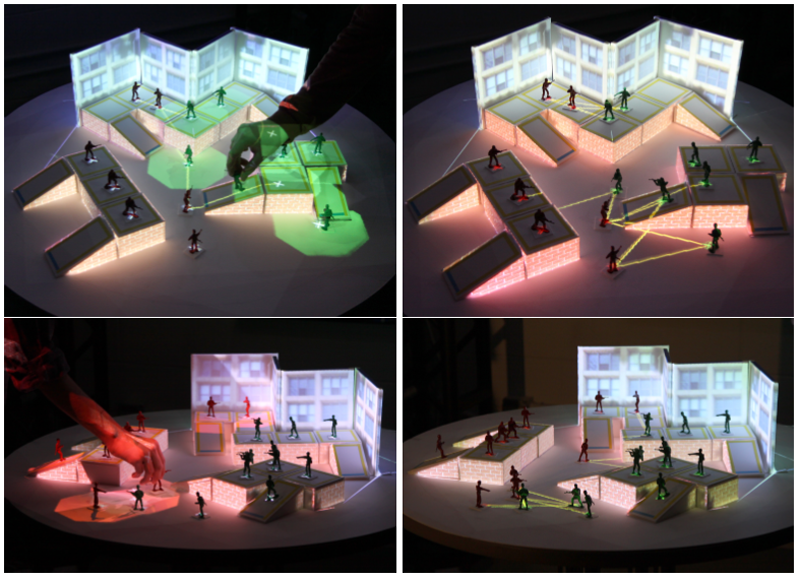
\includegraphics{army_screenshots}} \\
% \caption{ Imagery from Andrew Dolce's ARmy military simulation game
%   played on our Table Top Spatially Augmented Reality System.}
% \label{FIGURE_army_screenshots}
% \end{figure}
% 
% The participants position a set of small boxes, ramps, and partition
% walls made of lightweight white foamcore (foam+cardboard) and red or
% green plastic army units within the workspace to construct the 3D
% geometry of the game environment and control game play.  Images of the
% environment are captured by a camera mounted above the scene and are
% processed using computer vision to detect the current game state and
% create a 3D digital model.  The ARmy computer application calculates
% the legal movement range of each unit and also calculates the line of
% sight and distance between opposing units to determine if combat will
% occur between opposing units and if an advantage is afforded to one
% unit over the other because of elevation differences.  The projectors are used to
% directly augment the physical objects:
% \begin{itemize}
% \item adding realism to the environment by applying interesting textures
% to the surfaces (Figure~\ref{FIGURE_realism}),
% \item
%  visualizing the legal movement range (Figure~\ref{FIGURE_movement}), and
% %
% \item visualizing combat line of sight between opposing army units
% (Figure~\ref{FIGURE_combat}).
% \end{itemize}
% %
%  The computer also enforces the rules of the game
% (play is paused until illegal movements are corrected).
% 
% \begin{figure}[t]
% \centering
% \resizebox{2.5in}{!}{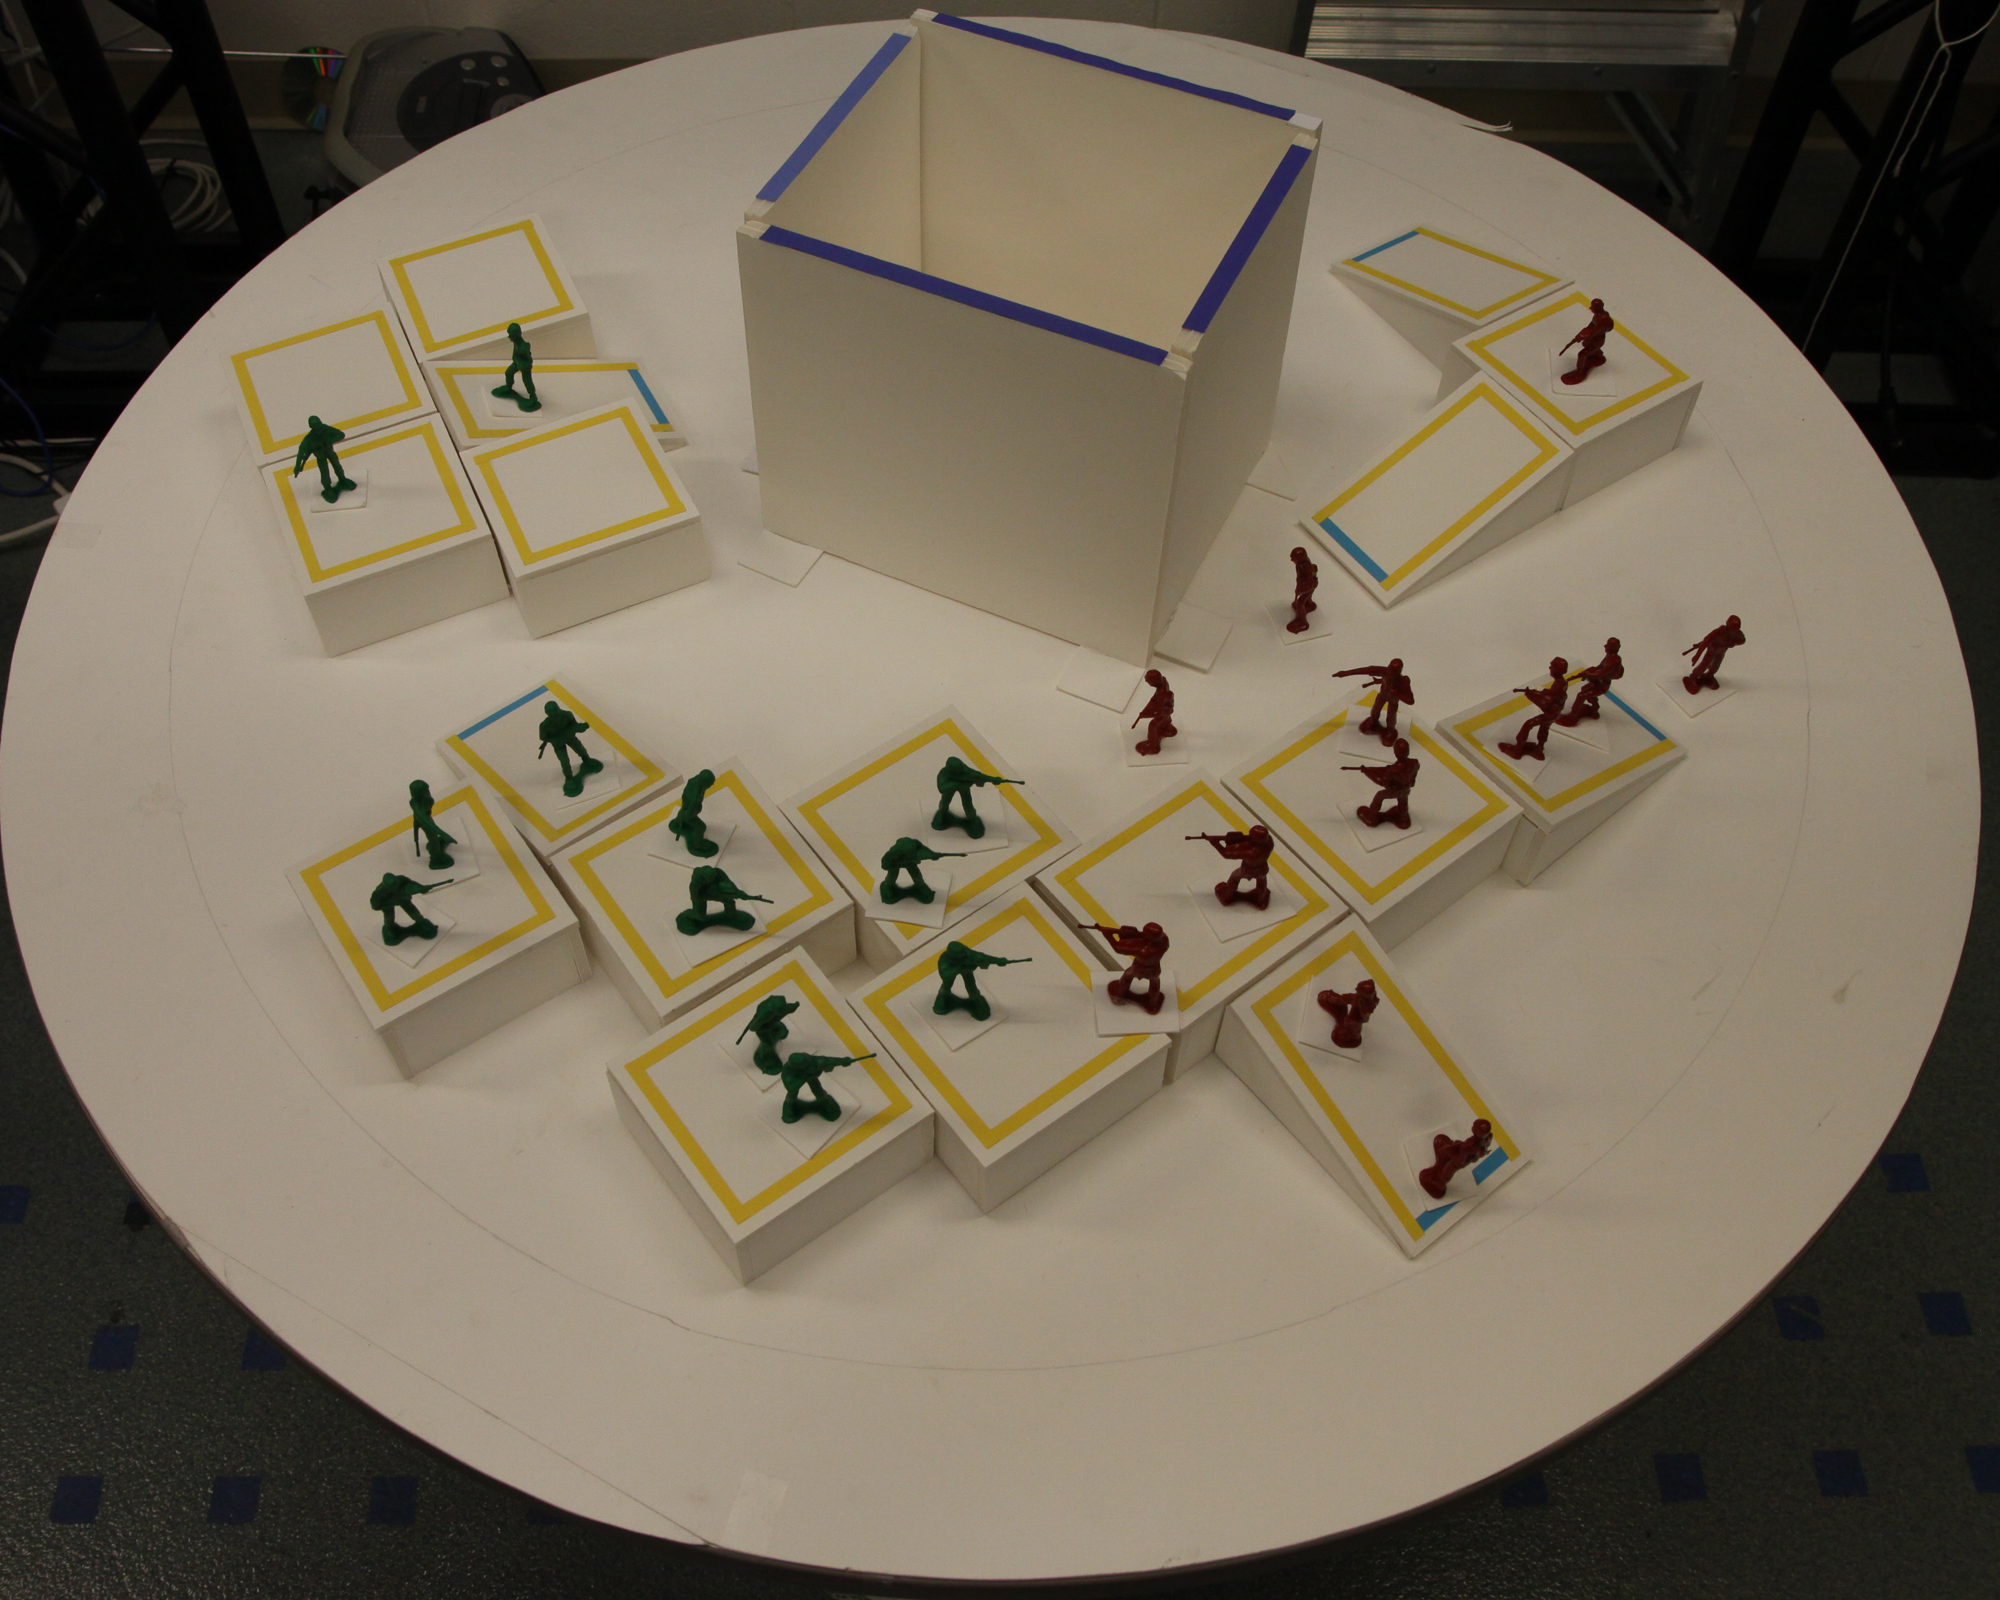
\includegraphics{complex_with_army_lights_on}}
% \resizebox{2.5in}{!}{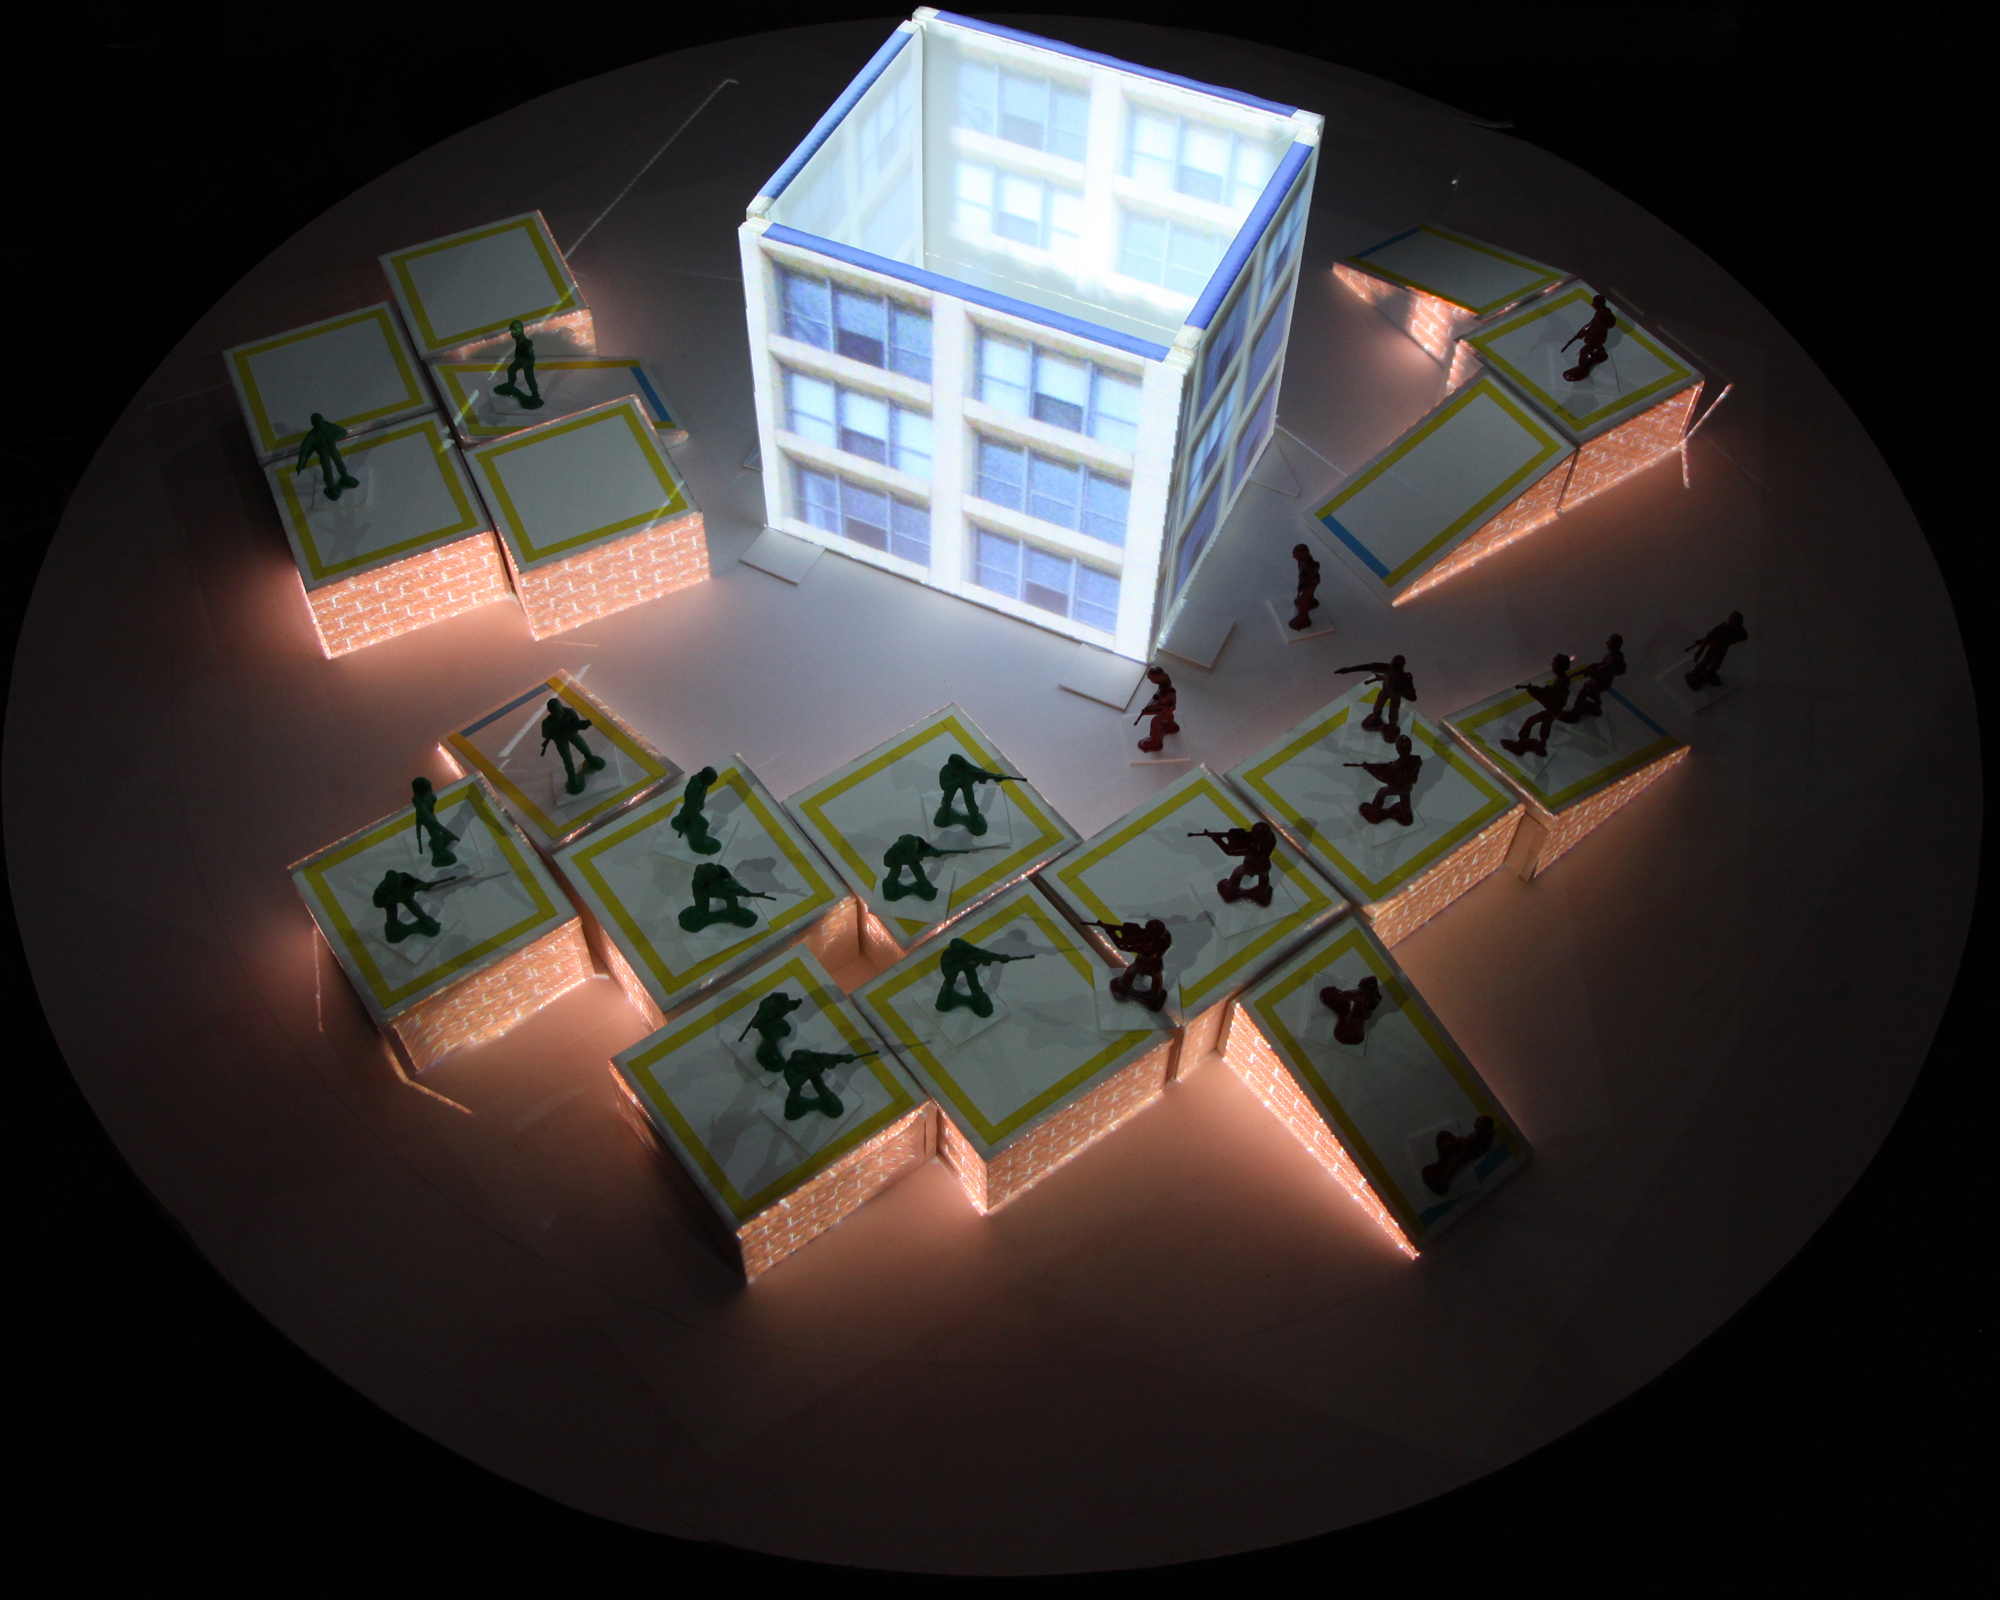
\includegraphics{complex_projection_with_army}} \\
% \caption{ The projectors are used to add realism to the plain white
%   surfaces by projecting simple building textures onto the physical scene.}
% \label{FIGURE_realism}
% \end{figure}
% 
% \begin{figure}[t]
% \centering
% \resizebox{2.5in}{!}{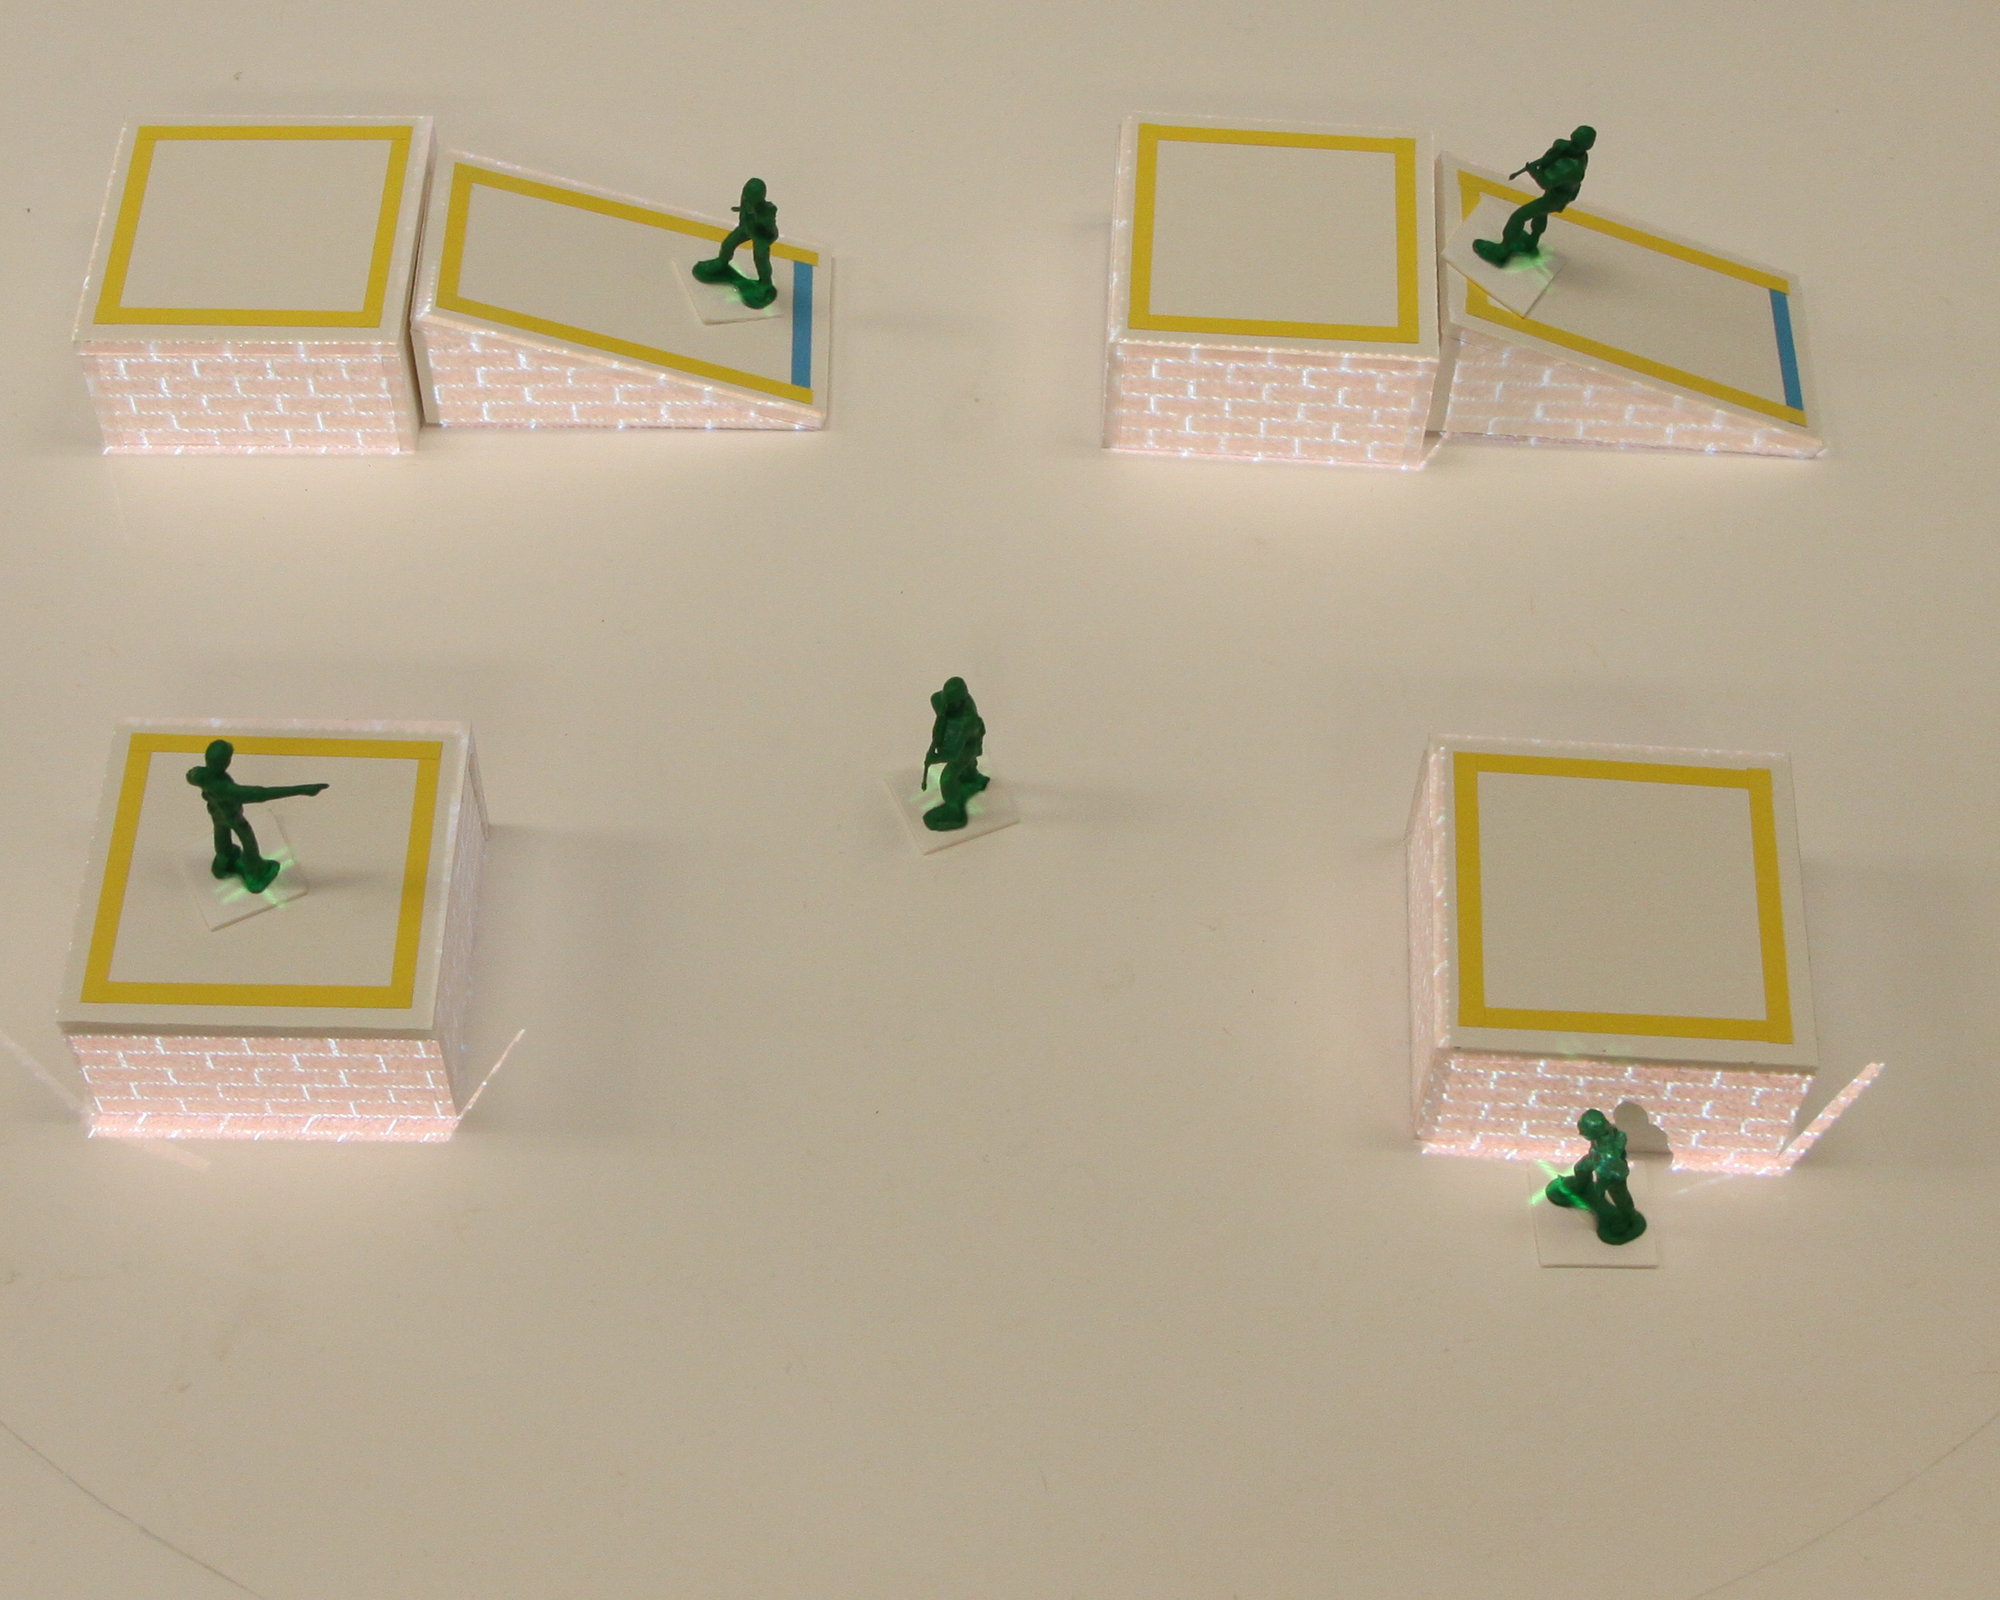
\includegraphics{movement_terrain_projection_lights_on_with_army}}
% \resizebox{2.5in}{!}{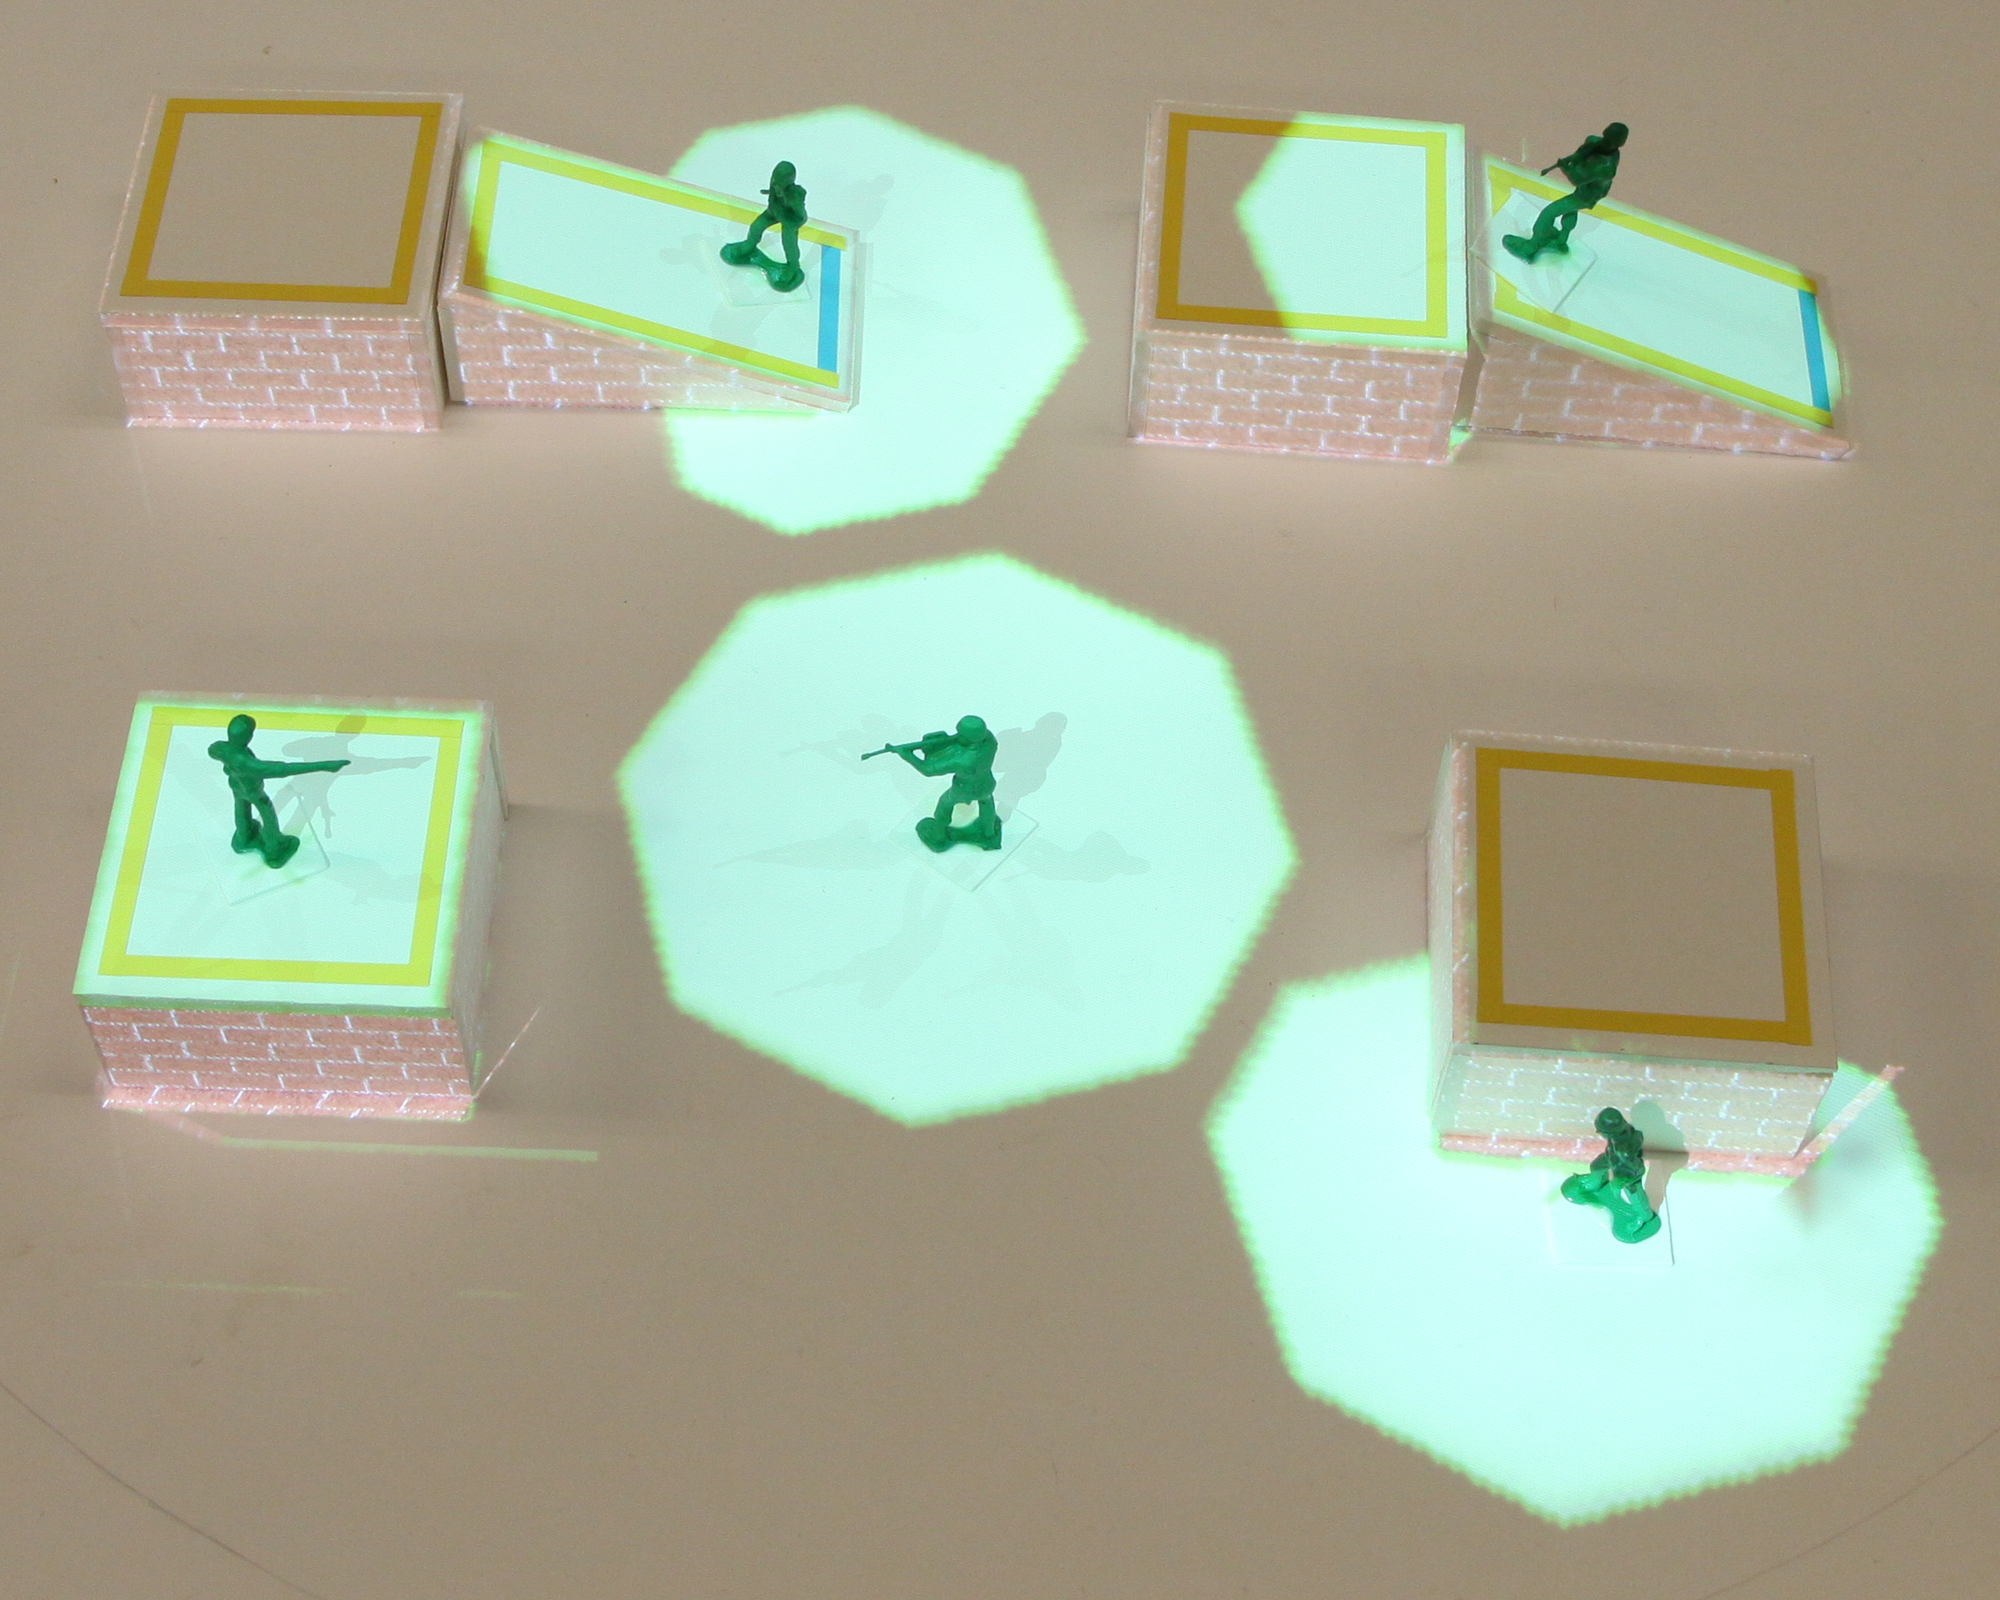
\includegraphics{movement_circles_projection_lights_on}} \\
% \caption{ The legal movement for each army unit is computed and visualized
%   directly on the physical scene using projection imagery.}
% \label{FIGURE_movement}
% \end{figure}
% 
% \begin{figure}[t]
% \centering
% \resizebox{2.5in}{!}{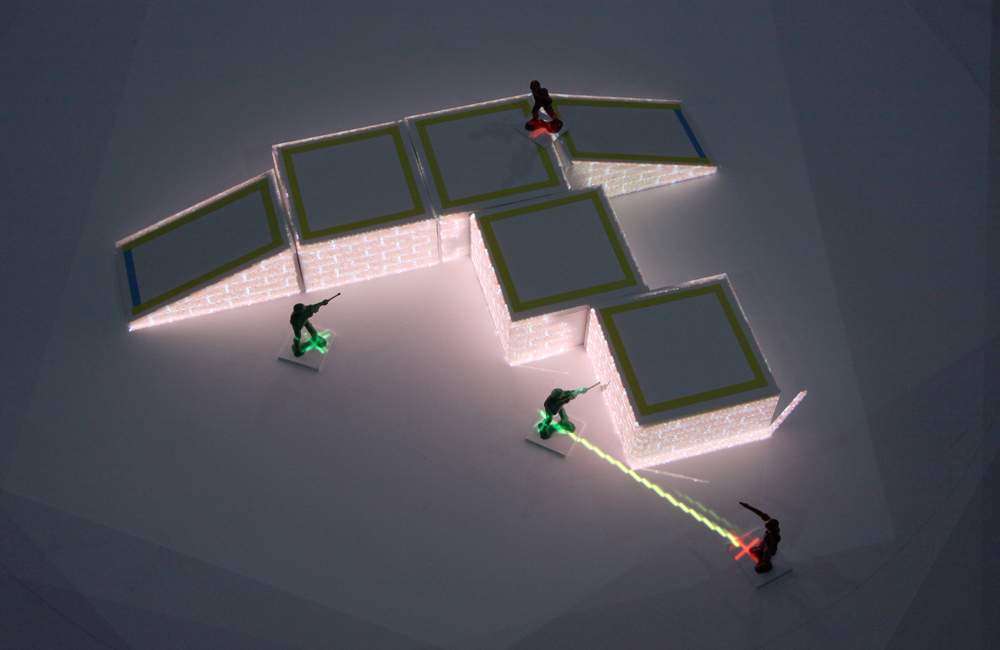
\includegraphics{combat_movement_u}}
% \resizebox{2.5in}{!}{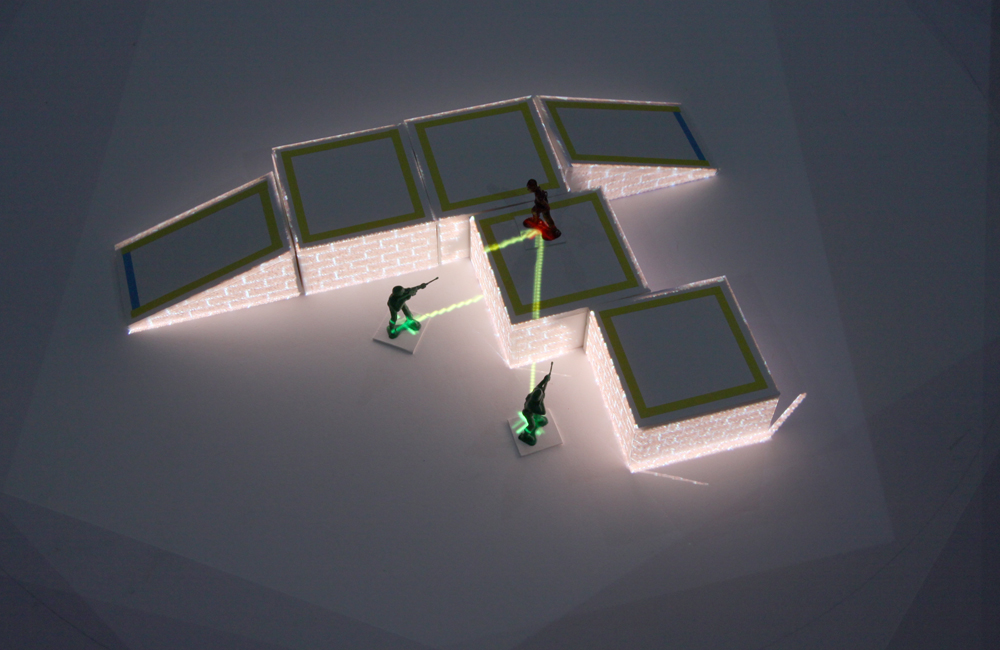
\includegraphics{combat_movement_ze}} \\
% \caption{ The line of sight between opposing army units is computed
%   and visualized by projecting yellow lines connecting army units that
%   are sufficiently close and do not have an obstacle between them. }
% \label{FIGURE_combat}
% \end{figure}
% 
% 
% 
% 
% 
% 
% 
% \begin{figure}[t]
% \centering
% \resizebox{!}{3.2in}{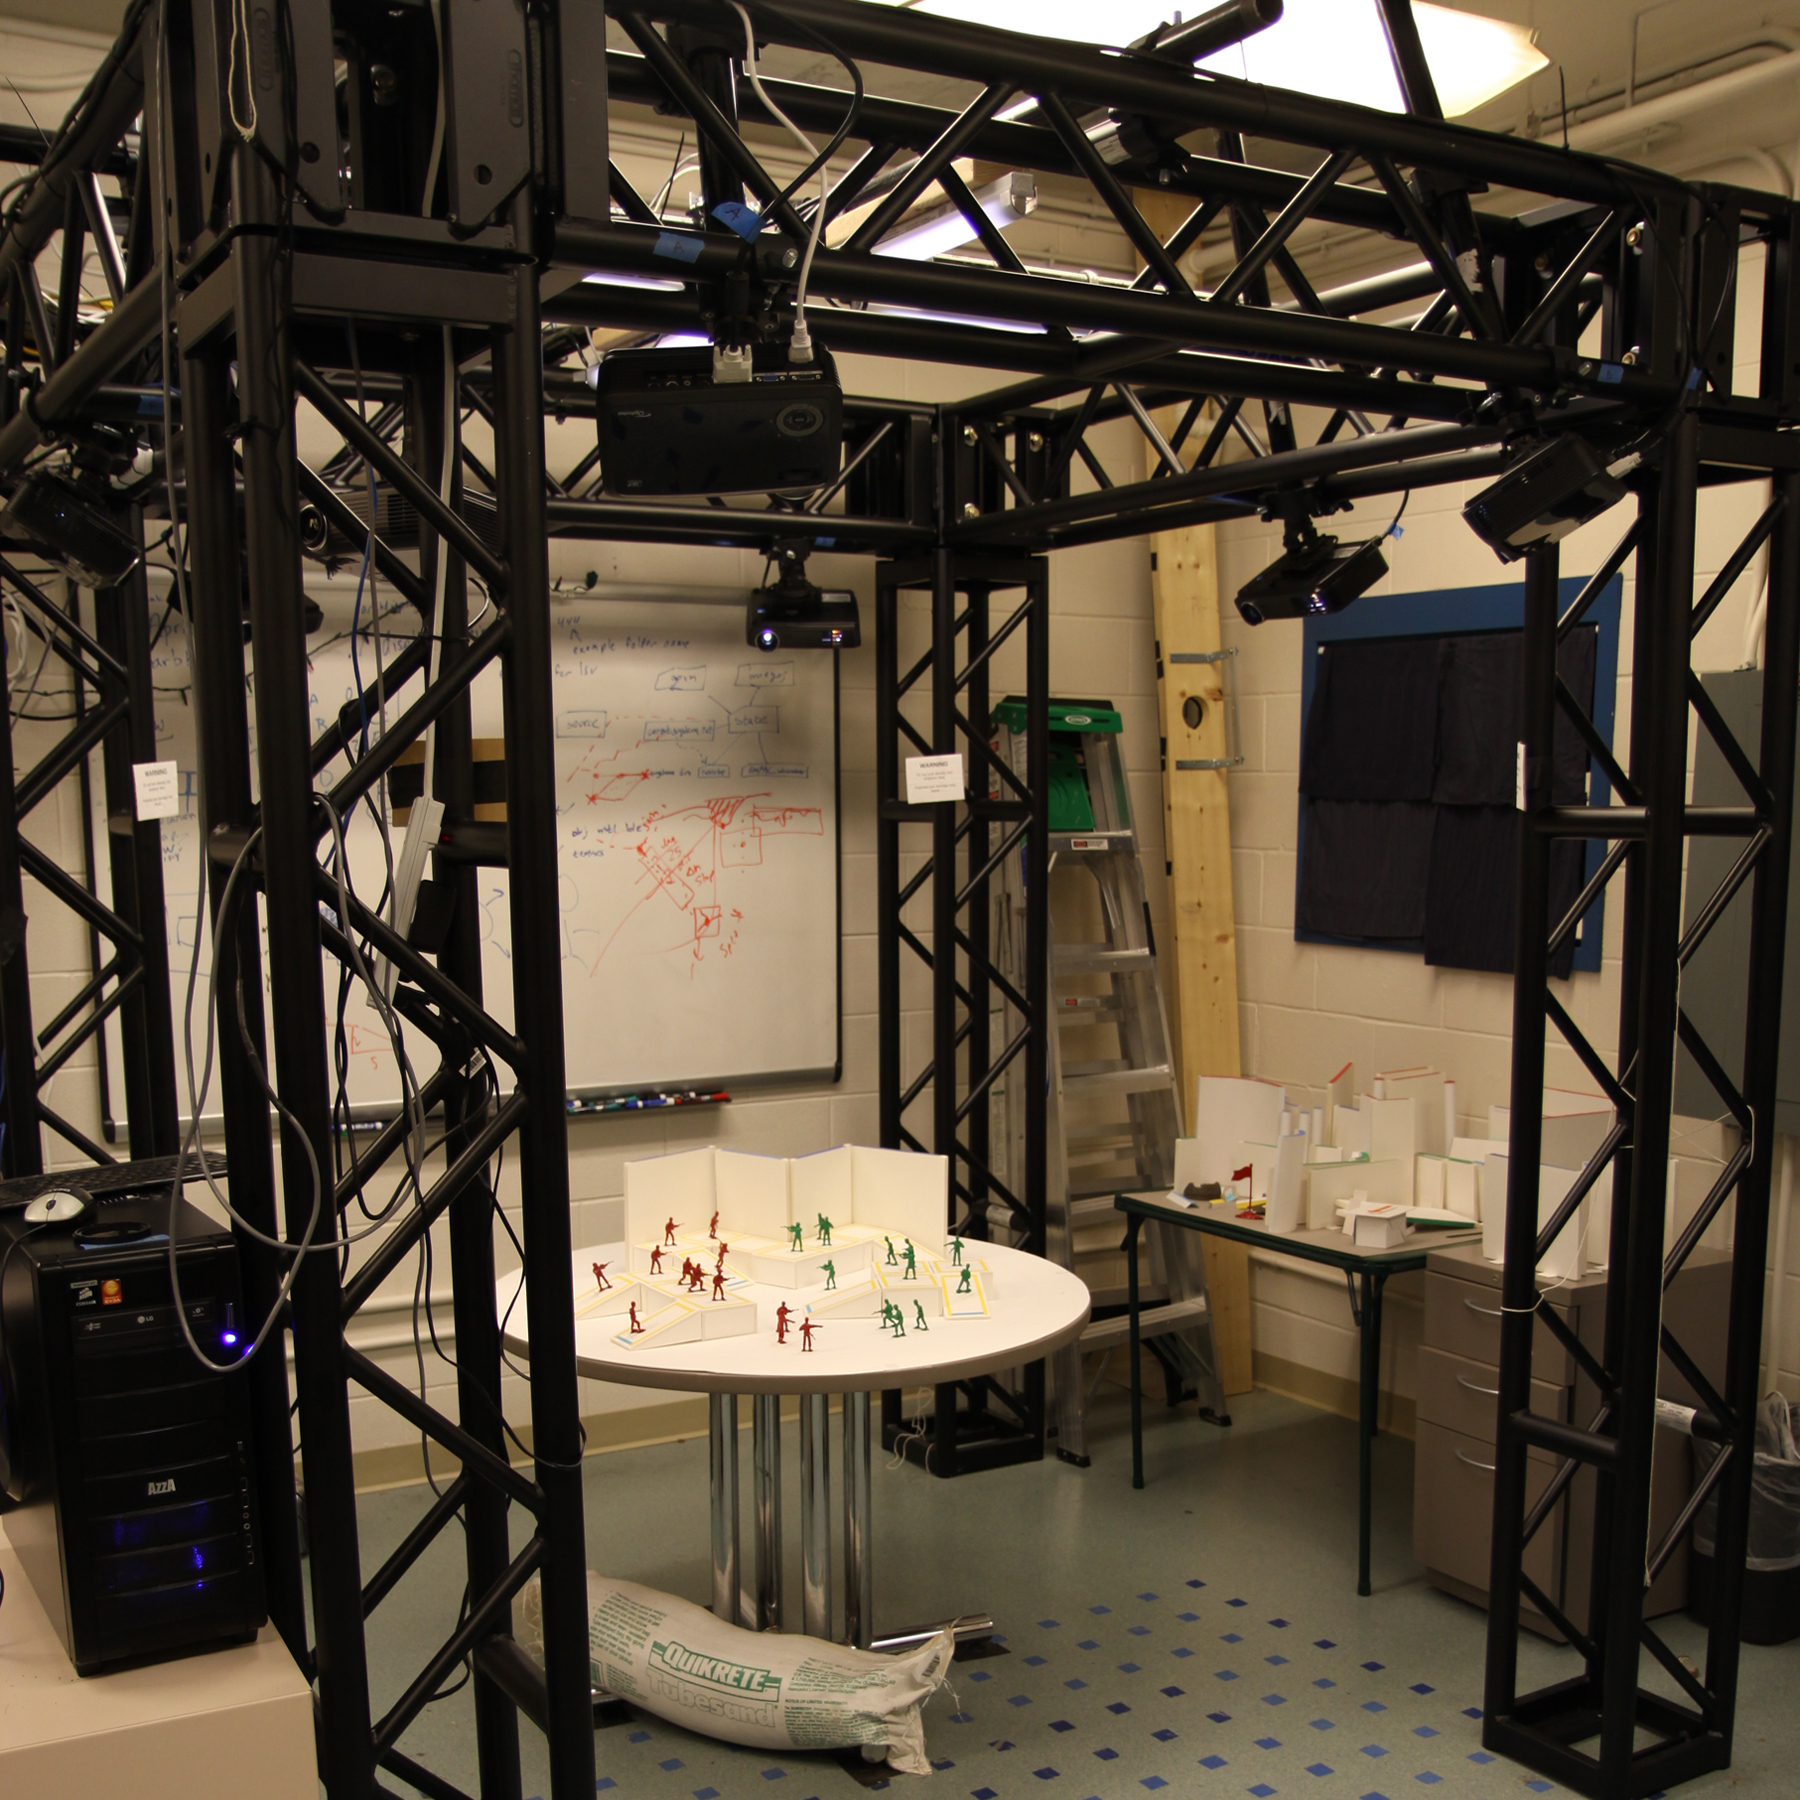
\includegraphics{contraption_frame}}
% \resizebox{!}{3.2in}{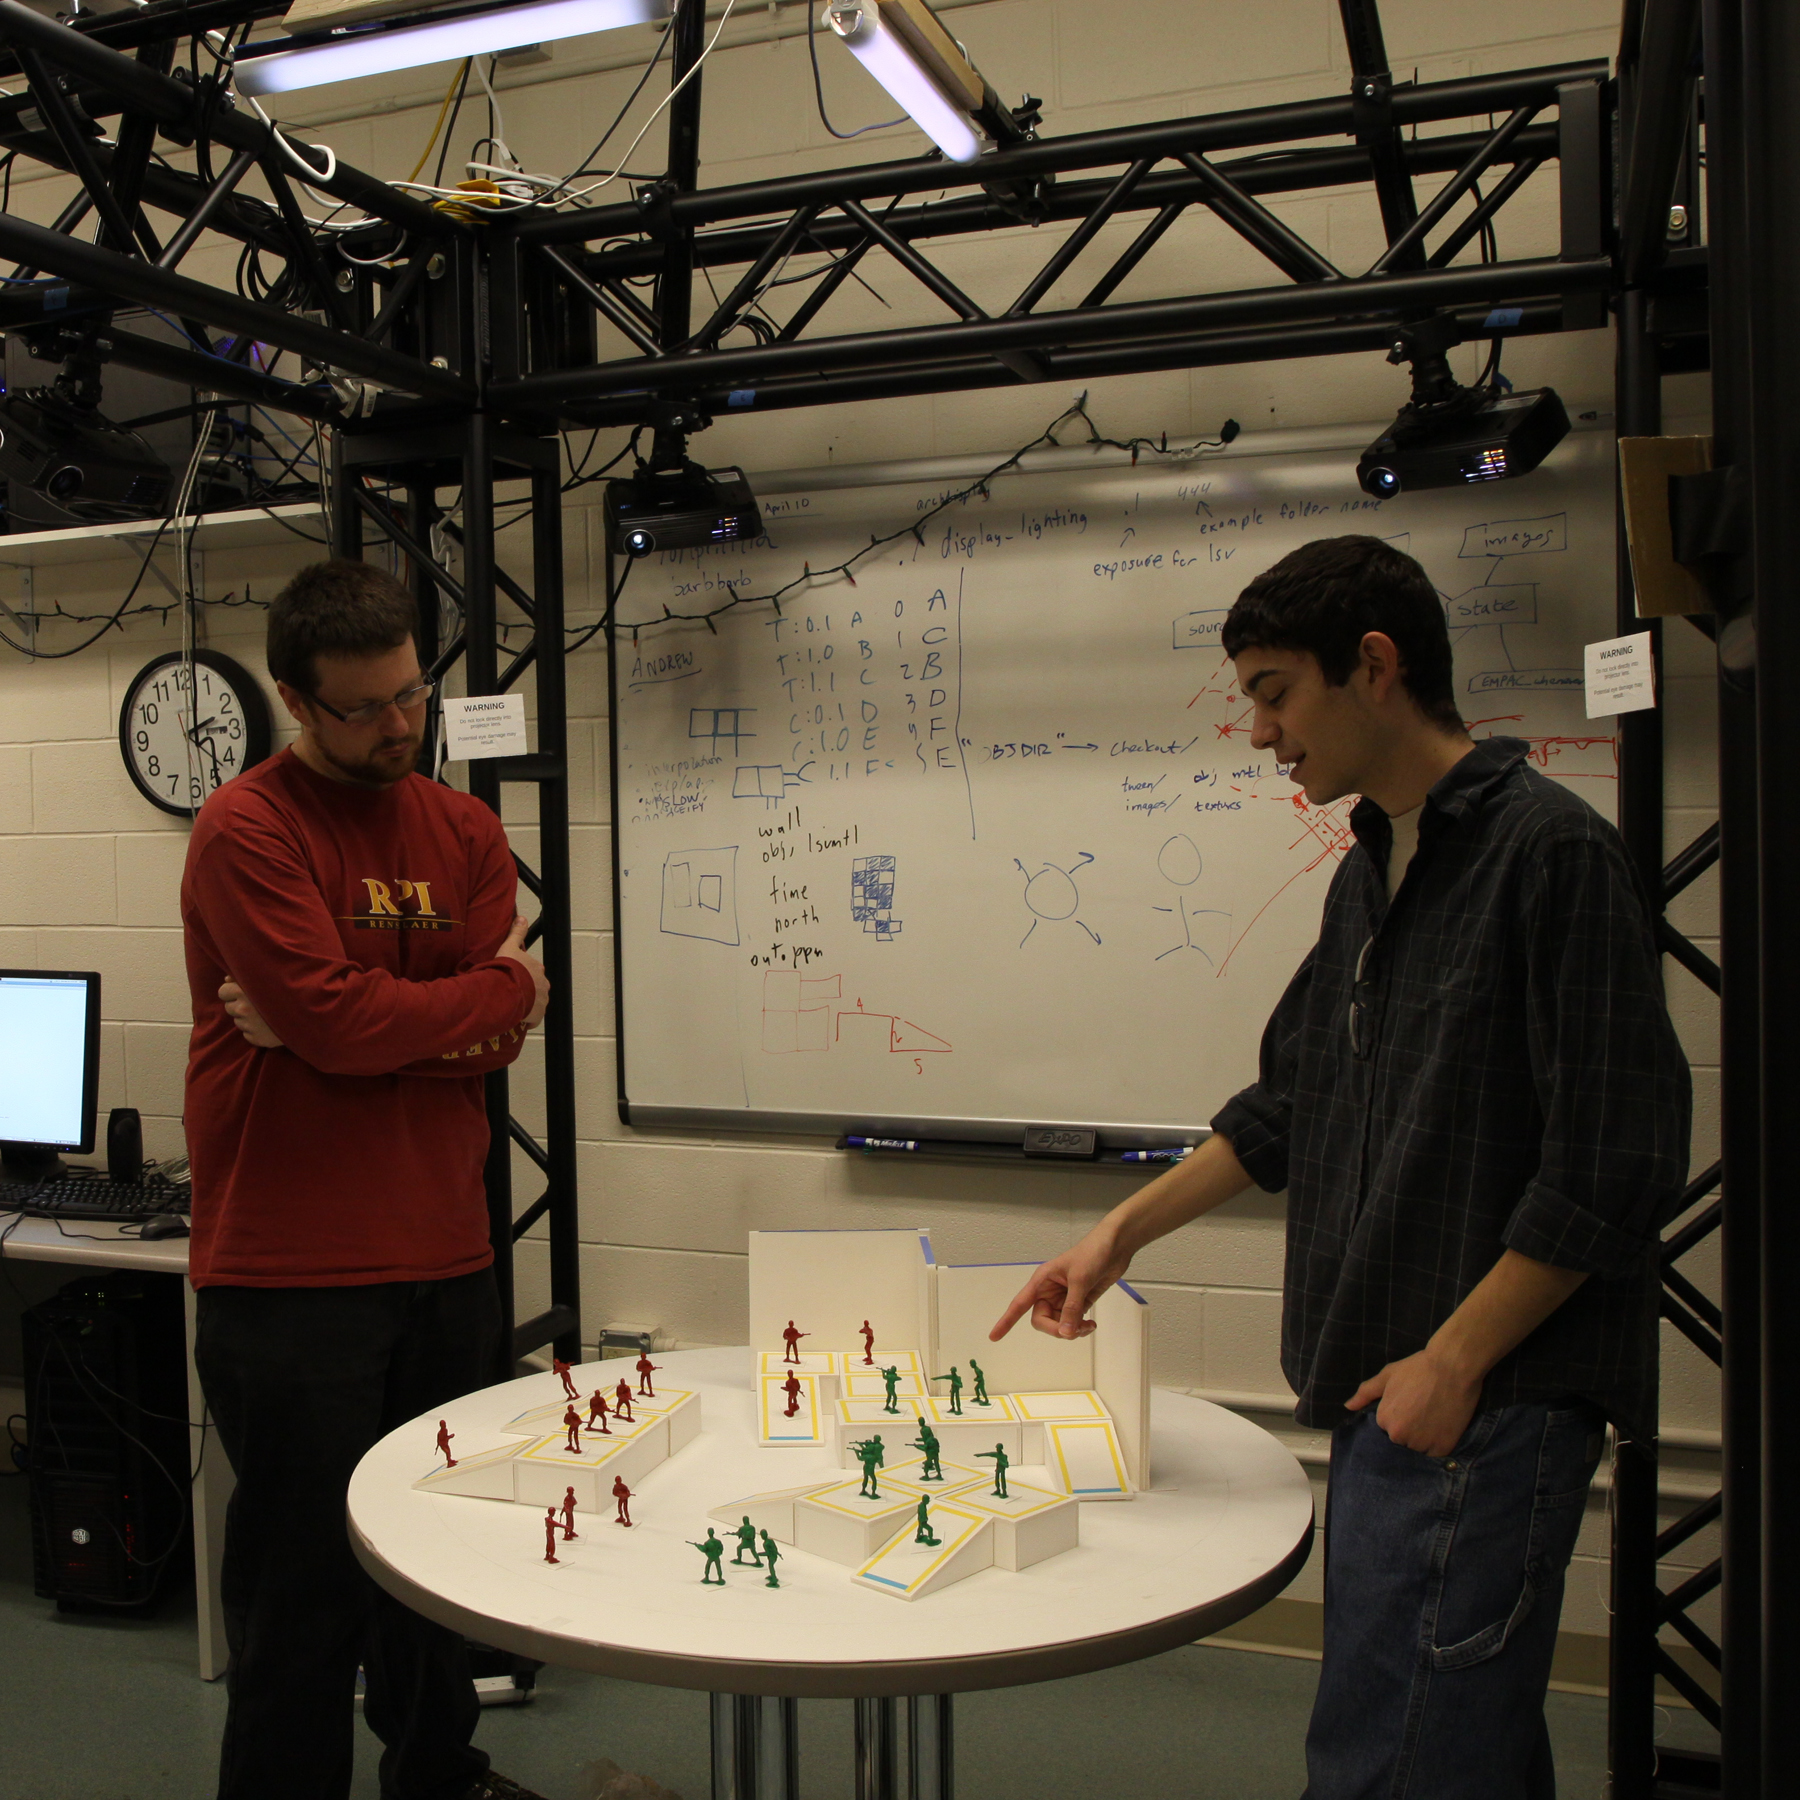
\includegraphics{contraption_with_people}} \\
% \caption{ The Table Top Spatially Augmented Reality System consists
%   of 6 projectors and 1 camera mounted on a frame of heavy-duty
%   aluminum truss frame commonly used in stage technology settings.
%   Users gather around a table in the center of the frame to play the
%   game and view visualization imagery projected on the 3D environment
%   built of white foamcore.}
% \label{FIGURE_contraption}
% \end{figure}
% 
% 
% 
% Our system (Figure~\ref{FIGURE_contraption}) centers around a standard
% 30'' high, 42'' diameter table.  A standard, heavy-duty stage
% technology aluminum truss frame positions the camera and projectors
% above the table.  The projectors and camera are securely mounted to
% the frame using appropriate, commercially-available mounting brackets.
% The wide stance of the frame allows more than 26'' of clearance
% between each of 4 vertical uprights and the table.  Three of the four
% sides of the frame are open with at least 3' of clearance.  The top
% bar of the frame is 7' above the base.  
% 
% Six standard portable office projectors (each weighing approximately
% 7.5 lbs) are mounted in a circle above the heads of the users using a
% standard mounting bracket rated to hold projectors of this size.  The distance
% from the floor to the bottom of the projector is over 6'6''.  A
% digital camera, weighing approximately 0.5 lbs, is positioned
% approximately 8' above the floor and is secured with a standard tripod
% mounting bracket.  Standard power and data cables are used to connect
% the projectors, camera, and lights to three computers placed on a desk
% near the frame.  The cables are neatly run along the upper bars of the
% frame and attached using cable ties and the excess cable is looped and
% secured next to the desk.  No cables are loose or are run along the
% floor.  The system contains no custom electrical components and all
% electrical components are used within their UL design specifications
% and according to the manufacturer's instructions.
% 
% Standard fluorescent tube room lighting is used during operation of
% the table top Spatially Augmented Reality system and will be used
% throughout the duration of the study.  The average illumination in the
% space is 300 lux (lumen/m$^2$).  For reference, recommended lighting
% levels for normal office and laboratory work is in the range of
% 250-1000 lux or for precision and detailed work the recommended range
% is 1500-2000 lux.  With room lighting only, the illumination on the
% table surface is 300 lux.  With all 6 projectors displaying full
% brightness white images, the center of the table surface is less than
% 20,000 lux.  For reference, noon sunlight falling on a horizontal
% surface is approximately 120,000 lux.  All objects that will be placed
% on the table are matte (not reflective or shiny) and thus the
% brightness from the projectors and halogen lights will be uniformly
% distributed in all directions and will not result in any intensely
% bright specular reflections to any viewpoint.
% 
% \begin{figure}[t]
%   \begin{center}
%     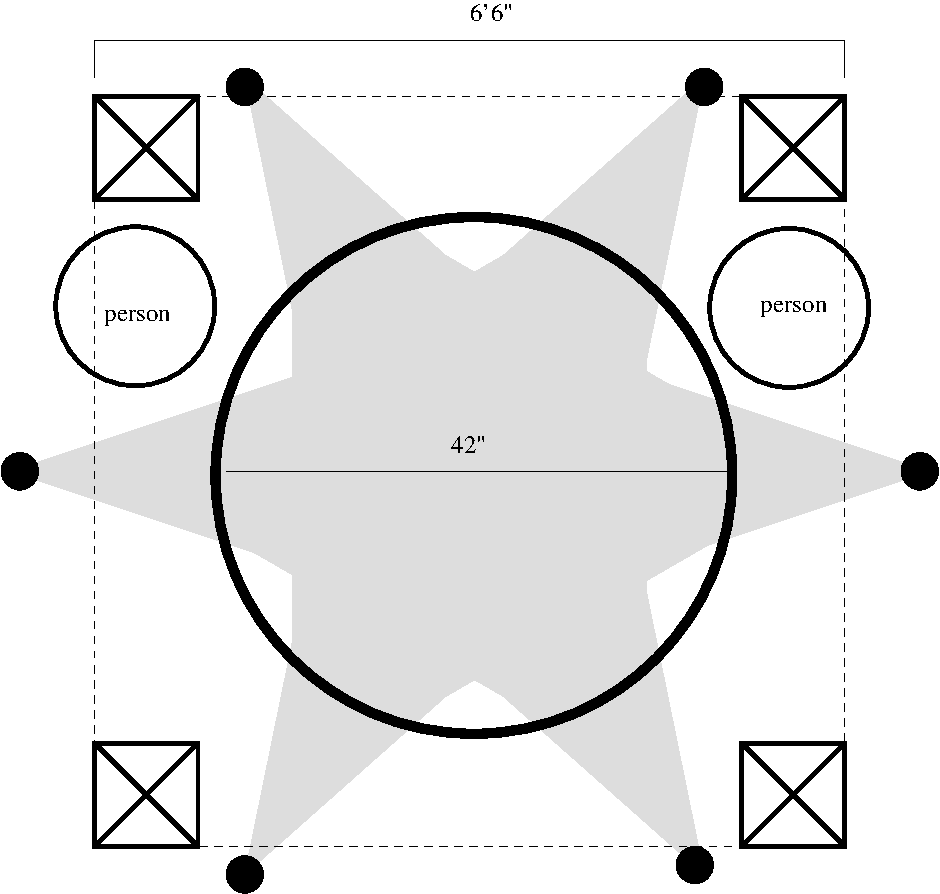
\includegraphics[width=0.45\textwidth]{top_view.pdf} \hfill
%     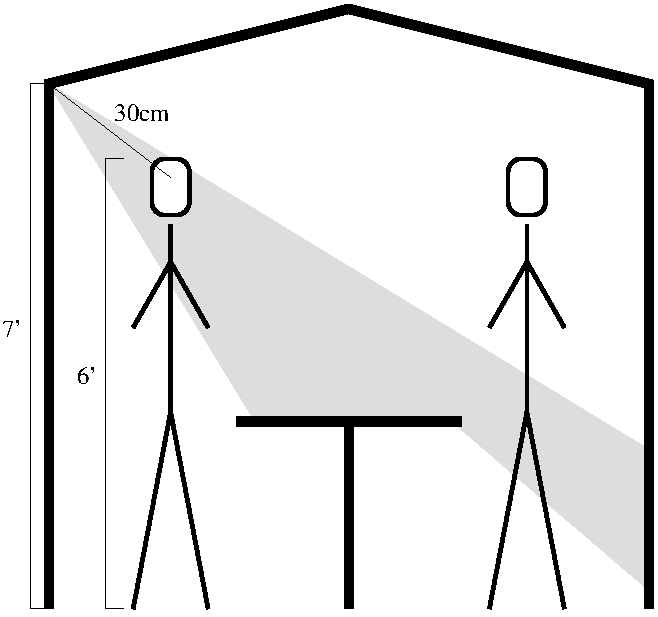
\includegraphics[width=0.5\textwidth]{side_view.pdf}
%   \end{center}
%   \caption{Diagram of system of system from the top (left) and side
%     (right).  The natural place for users to stand during use of the
%     system is next to the table between two uprights rather than
%     between the table and one upright as this would put them in the
%     beam of light and cause shadows on the table. The natural gaze of
%     participants is downwards towards the table or horizontally to
%     make eye contact with other users rather than directly into the
%     projector lens.
% \label{FIGURE_system_diagram}
% }
% \end{figure}
% 
% \section{Safety of Projectors}
% 
% We are using 6 Optoma EP 727 projectors.  Each projector uses a 180W
% Phillips UHP mercury lamp.  These projectors are typical small
% portable projectors that are used for everyday presentations.  We have
% not made any physical modifications to the case of the projector, thus
% all manufacturer safety features to protect users in the event of a
% bulb failure or breakage are still in place.  Similarly, we have not
% made any modifications to the intensity of light output from the
% projector or removed or changed any of the filters and lenses
% installed in front of the bulb.  Thus, intuitively, because it is safe
% to observe (for extended periods of time) the screen upon which the
% image is projected, logically it is also safe to observe the table and
% wall surfaces upon which these projectors display images.  We further
% analyze this safety in the following section.
% 
% It is not recommended to stand in the beam of projection and look
% directly at the projector.  Use of our system and our specific user
% studies will never require or ask the users to gaze toward the
% projector lens (Figure \ref{FIGURE_system_diagram}) and we will
% caution them both verbally and through signage about the potential
% eye hazard in doing so (Figure~\ref{FIGURE_warning_signs}).  However,
% we note that during normal use of these and similar projectors for
% class or office presentations, the presenter often does just this as
% he faces the audience.  Thus, our system is well within the normal,
% expected, and safe use of these devices.
% 
% 
% \begin{figure}[t]
%   \begin{center}
%     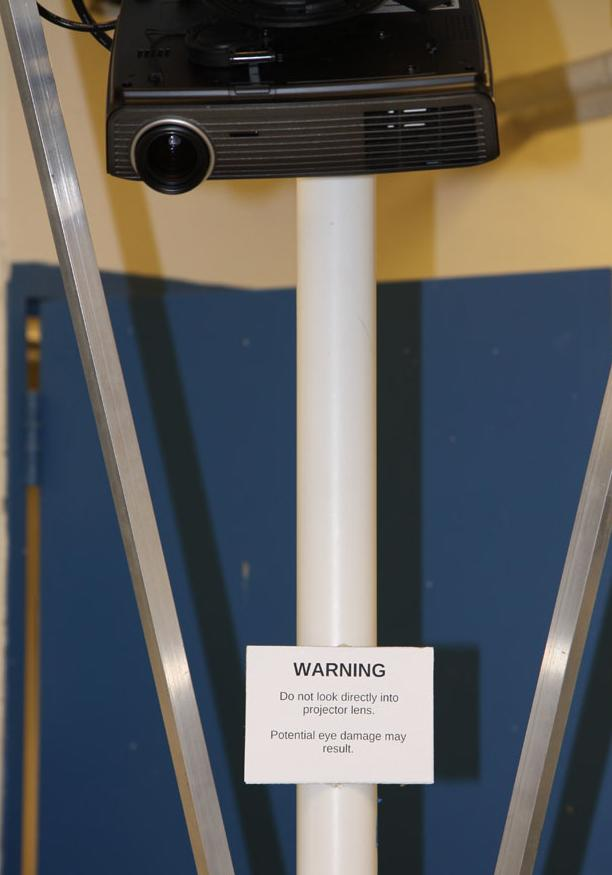
\includegraphics[width=0.3379\textwidth]{img_1193_small2.jpg}
%     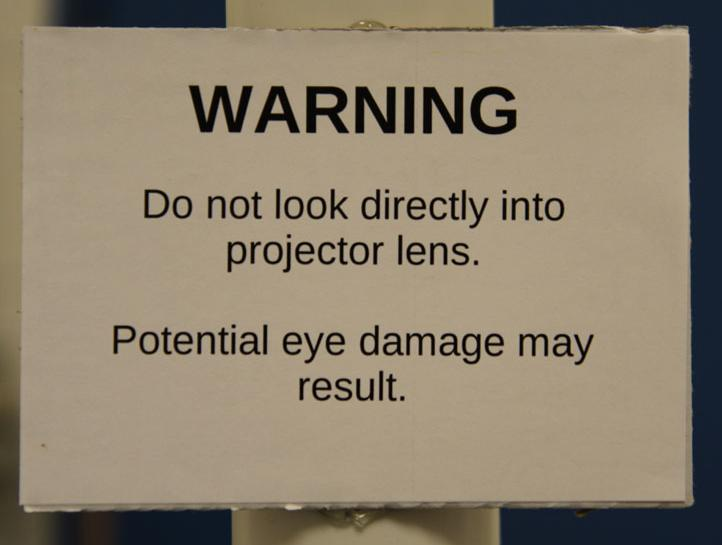
\includegraphics[width=0.64\textwidth]{img_1194_small2.jpg}
%   \end{center}
%   \caption{In addition to verbally instructing participants to avoid
%     looking into the projector lens, we have installed warning signs
%     near each projector at eye level, in a clearly visible position.
% \label{FIGURE_warning_signs}
% }
% \end{figure}
% 
% 
% We made a concerted effort to obtain safety documentation on the
% intensity and spectral distribution of the light from this specific
% bulb directly from the manufacturer and distributor.  We contacted
% both Optoma and Phillips in December 2008 asking for the Spectral
% Power Distribution (SPD) of the equipment we have purchased from
% Optoma (the bulb is apparently manufactured by Phillips).  Both
% companies replied within a few days and we were told that the
% information was not available.  A second request to Phillips for the
% same information was made on May 4th 2009.  We called 1-800-937-5483
% and were told that ``UHP'' in the name of the lamp indicated that the
% bulb was an OEM part, thus the data was not available.  She suggested
% that we contact Optoma for the data.  She did give us the number of
% the OEM division of Phillips (1-866-915-5886).  From the OEM division,
% we were transferred to Technical Assistance, who spent about 30
% minutes searching for the specifications, but they were ultimately
% unable to locate the bulb (or any 180W projector lamp) in their
% equipment catalog.
% %
% %They gave us the
% %number of a specialty lamp division at Phillips (1-732-563-3339) and
% %...
% A second request to Optoma was made through their website on May 4th,
% 2009.  The auto-reply email said we would here from a technical
% specialist within 24-48 hours, but we have not heard a response.  
% 
% Since we were not able to obtain the information directly from these
% companies, we were forced to make these measurements and safety
% calculations ourselves.  
% 
% %Using the SPD data and the table of the ``Spectral Weighting Functions
% %for Assessing Retinal Hazards from Broad-Band Optical Sources'' the
% %Blue Light Hazard Exposure Limits can be calculated [ANSI/IESNA
% %  RP-27.1-05].  
% 
% %We attempted to borrow a spectroradiometer, equipment that can measure
% %the SPD, to directly measure the quantity and distribution of light
% %from these devices during normal operation.  Unfortunately,
% %Dr. Mariana Figueiro in the RPI Lighting Research Center said her lab
% %did not have equipment we could borrow.  Similarly, Dr. E. Fred
% %Schubert of the Future Chips Constellation said his lab did not have
% %any equipment capable of making these measurements.
% 
% 
% \section{Blue Light Hazard Calculation Detail}
% 
% To evaluate the retinal photochemical hazard posed to study
% participants by light emitted by the six projectors used in the
% system, we calculated permissible time limits for exposure during an
% eight-hour period in accordance with ANSI/IESNA RP-27.1-05,
% specifically section 4.3.2, ``Retinal Blue Light Hazard Exposure
% Limit.''  Two calculations were performed: exposure limits for the
% system as it is intended to be used (study participants looking at
% matte white surfaces illuminated by up to six projectors), and
% accidental direct viewing of the lens of one projector from within the
% beam of that projector.
% 
% During the intended use of the system, study participants will view
% matte-surface card-stock and foam-core board illuminated by up to six
% projectors.  For purposes of hazard evaluation, we assume 100\%
% reflectivity (measured at 95\%) and Lambertian reflectance
% characteristics.  We assume all six projectors are illuminating the
% table in a direct-incidence configuration, which is a worst-case
% situation, although not physically possible with the system
% (projectors are rigidly mounted in opposing directions).  Moreover, we
% assume that all six projectors produce the same spectral irradiance
% at the table surface, and take this irradiance to be the maximum
% measured over all six projectors (output varies due to bulb
% manufacturing tolerances and degradation over bulb lifetime).
% 
% \begin{figure}[t]
%   \begin{center}
%     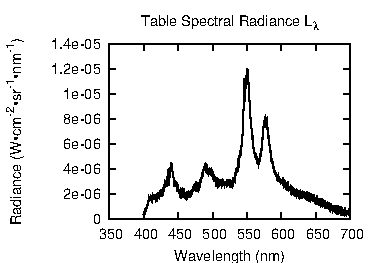
\includegraphics[width=0.6\textwidth]{table_radiance.pdf}
%   \end{center}
%   \caption{Measured worst-case radiance from table surfaces.
% \label{FIGURE_worst_case_radiance}
% }
% \end{figure}
% 
% We measured the relative spectral output of the projectors with an
% Ocean Optics spectroradiometer and calibrated the measurements at the
% table surface to spectral irradiance ($W/m^2\cdot nm$) using a
% calibrated luxmeter with accurate CIE $V_m(\lambda)$ characteristics
% (Figure~\ref{FIGURE_worst_case_radiance}).  We evaluated the
% blue-light hazard function according to the following equation
% \cite{ANSI}:
% 
% 
% \[L_B = \sum_{300}^{700}L_{\lambda}\cdot B(\lambda)\cdot \Delta \lambda\]
% 
% Given the worst-case assumptions presented above, we calculated a
% blue-light hazard weighted radiance reflected from the table of
% $1.73\times10^{-4}$ $W/cm^{-2}\cdot sr^{-1}$.  This value is less than
% 2\% of the maximum allowed for time exceeding $10^4$ seconds (2.77h)
% \cite{ANSI}, a period substantially longer than the maximum 1.5 hour
% study participants will be allowed to use the system.  We conclude
% that there is no retinal photochemical injury hazard from the intended
% use of the system.
% 
% Due to the design of the system, it is possible for study participants
% to accidentally look directly into the projector.  To evaluate this
% hazard, measurements were taken of the spectral radiance of the
% projectors at a distance of 30cm from the projector lens, which is the
% closest the eyes of a 6'-tall individual can get (measurements
% obtained with projectors off). At this distance the blue light hazard
% weighted radiance is $L_B = $ 43.2 $W/cm^{-2}\cdot sr^{-1}$. According
% to the formula \cite{ANSI}:
% 
% \[t(max) = \frac{100}{L_B},\]
% 
% \noindent
% the maximum permissible exposure is 2.3 seconds.  Since the perceived
% brightness of the projectors at this distance is comparable to that of
% direct noon sunlight, it is doubtful that study participants would
% accidentally stare directly into the projectors for extended periods
% of time, since we expect that this would be uncomfortable, and the
% natural reaction would be to look away and step out of the projector
% beam.  To mitigate the risk presented by possible exposure several
% steps will be taken.  First, study participants will be instructed
% both verbally and in writing not to look directly into the projectors
% since this may cause eye damage.  Additionally, warning signs have
% been posted (Figure~\ref{FIGURE_warning_signs}) in a clearly visible
% location near each projector warning participants of possible eye
% damage and instructing them not to look directly into the projector
% lenses.  Finally, during the study the person running the study will
% carefully monitor the participant and if the participant's gaze is
% drawn away from the table for an extended period, they will be
% encouraged to step completely away from the SAR frame to prevent
% accidentally gazing into the projector lens.
% 
% As a verification of our measurement and calibration procedures, we
% ran identical calculations for noon sunlight and obtained maximum
% per-day exposure limits within 10\% of published results
% \cite{Okuno08}.
% 
% 
% 
% 
% 
% 
% 
% 
% \begin{thebibliography}{widest entry}
%   \bibitem{Okuno08} Okuno, Tsutomu, ``Hazards of Solar Blue Light,'' Applied Optics, V. 47,
%     No 16. June 1, 2008.
%   \bibitem{ANSI} ANSI/IES RP-27.1-05, ``Photobiological Safety for Lamps and Lamp Systems -
%  General Requirements,'', Illuminating Engineering Society, 2005.
% \bibitem{dolce}
% Dolce, Andrew, 
% ``Multi-User Interactions for Spatially Augmented Reality Games''
% Masters Thesis, Rensselaer Polytechnic Institute, 
% Department of Computer Science,
% June 2011.
% \url{http://www.cs.rpi.edu/graphics/theses/andrew_dolce_MS_May2011.pdf}
% \end{thebibliography}
% 


\newpage

\pagestyle{empty}

\begin{center}
{\Large {
Institutional Review Board \\ \vspace{0.1in}
Rensselaer Polytechnic Institute} }\\
\ \\
{\large Informed Consent Form}
\end{center}

\noindent
I understand that Barbara Cutler, who is a professor of Computer
Science at Rensselaer Polytechnic Institute, and Tyler Sammann, a Computer
Science Master's student at Rensselaer Polytechnic Institute, would like me to use a
new sound interface and answer a short questionnaire as part of the
research project on a new multi-user collaborative system for sound
and music editing for Tyler Sammann's research.  I understand that they
will be making their best possible effort to guarantee me every possible
protection, including the following:

\begin{enumerate}

\item I am 18 years or older.

\item
I am under no obligation to be participate in the study or to be
  complete the questionnaire if I do not wish to do so.

\item 
I am not obligated to perform any of the exercises or
  answer any of the questions.  I may decline to answer any or all of
  the questions, and I may terminate the study at any point, without
  giving any reason.

\item 
There will be no monetary compensation for my participation in this 
study. 

\item I will be identified by a randomly assigned ID number that is
  used only for this study.  All recordings and log files will be
  labeled with this ID.  All information and data relating to the user
  study will be protected to secure confidentiality.  All electronic
  files will be stored on password protected computers.  All paper
  forms will be stored in a locked office.  The correspondence
  between the ID number and my name will be recorded by Barbara Cutler
  and be accessible only by her.  This correspondence will be
  destroyed once analysis of the data is complete, within 1 year after
  participation in the study.

\item  The interaction session
  may be recorded with a simple video camera (positioned behind users, 
  capturing the players backs and not their faces). 
  The players voices will also be recorded.  The audio
  recordings will not be used, but quotations from the recordings may
  be extracted as samples in the thesis documentation. The video/audio recording
  will be destroyed within 1 year after participation in the study.\\
\noindent
\hspace*{0.3in} \rule{0.3in}{1pt} I agree to be video and audio taped. \\
\hspace*{0.3in} \rule{0.3in}{1pt} I do not agree to be video and audio taped.

\item System audio produced and created as a result of using the interface will 
  be recorded and saved as digital files for later analysis. Mouse and keyboard
  motion and interactions will also be logged and saved for later analysis.
  The logged mouse and keyboard interaction data may be used in the thesis document.
  The system audio recordings will not be used in the thesis documentation. These
  data files and recordings will be destroyed within 1 year after participation
  in the study. Within this time, and with the permission of all users in the study,
  recorded system audio files will be released to participants upon request.\\
  \noindent
\hspace*{0.3in} \rule{0.3in}{1pt} I agree for my mouse and keyboard actions to be logged and saved. \\
\hspace*{0.3in} \rule{0.3in}{1pt} I do not agree for my mouse and keyboard actions to be logged and saved.\\
\\
\hspace*{0.3in} \rule{0.3in}{1pt} I agree for system audio to be recorded and saved. \\
\hspace*{0.3in} \rule{0.3in}{1pt} I do not agree for system audio to be recorded and saved.\\

\end{enumerate}

\vspace{0.3in}

\begin{center}(continued on next page)\end{center}

\newpage

\begin{center}(continued from prev page)\end{center}

\vspace{0.3in}

\begin{enumerate}
\setcounter{enumi}{8}

\item Sounds in the study environment will be limited in the system to a loudness of
  85 dB(A), and loudness will be monitored with a sound level meter during the study. 
  Permanent hearing damage can occur if listening to prolonged sound or noise
  at 85 dB(A) for 8 hours or more. If at any time I become uncomfortable with the 
  loudness, or any other part of the study, I may request for the master volume to be
  lowered. I may also request for the sound to be muted and/or the experiment stopped at
  any time. I am also free to leave the study at any time.
  
\item If there is anything that I do not wish to have quoted, or any
  interface state files that I do not want made public, I may say at any
  point during or after the study what I wish to have kept off the
  record and it will not be quoted or used in a publication or thesis document.

\item I understand that if Barbara Cutler or Tyler Sammann decides to use any portions
  of my answers to the questionnaire or any examples of my system interaction
  documentation or verbal comments during system use in subsequent publications, that
  they will send me a copy of the portions of the questionnaire and any
  interaction documentation, including any quotations and paraphrases that she decides
  to use, for my editing and written approval. I will have the right
  to edit the material and I will have access to the final publication. They
  will only use the material that I have approved and the use of all
  material will be anonymous. I may also change my mind at any point
  up to and including the review of any quotations and paraphrases and
  interaction documentation that might be used.

\end{enumerate}

\vspace{0.5in}

\noindent
\rule{2.6in}{1pt}~~~~\rule{2.6in}{1pt}\hfill \rule{1in}{1pt}\\
\hspace*{0.7in}Name of Participant 
\hfill Signature \hspace{1.3in} 
Date \hspace{0.3in}

\vspace{0.15in}
\noindent
For further information contact:

%\vspace{0.05in}
\noindent
Barbara Cutler, Department of Computer Science, MRC 330B, cutler@cs.rpi.edu,\\
110 8th Street, Troy NY 12180; phone: (518) 276 3274, fax: (518) 276 2529.

%\vspace{0.05in}
\noindent
Institutional Review Board, Rensselaer Polytechnic Institute, CII 9015, \\
110 8th Street, Troy, New York, 12180; phone: (518) 276-4873, fax: (518) 276-4002.
\vspace{-0.8in}

\newpage

\noindent
{\bf {\Large Sample Multi-User Collaborative Sound Interface Instructions}}

\vspace{0.2in}
\noindent
After receiving the system introduction and safety safety
instructions, the basic guidelines and instructions for the study 
are provided to the participants:

\begin{enumerate}

\item The user with the guitar will provide the input sounds to the 
  current system. They will not have a mouse. They will not be able to 
  make edits or modifications in the system.

\item Every other user will have a USB mouse. These users will not play any 
  instruments, or provide input sound, but will be able to use their mouse
  to make modifications and edit the sounds with the interface.
  
\item There will be two different sessions, and in each session the participants
  will use a different interface. One of the interfaces will be the well established
  digital audio workstation, Audacity. The other will be our new multi-user collaborative
  user interface. 
  
\item Goals for the session are guidelines, and exploring the possibilities of each
  interface is encouraged.
  
\item As much as possible, collaborate with your other group members. The ``editor'' users
  should be talking amongst themselves to make changes. Even more important is the communication
  and collaboration between the ``editors'' and the ``player.'' The player will likely have
  ideas about how to edit their recordings, and the ``editors'' will need to communicate with
  the ``player'' in order to achieve the kinds of input recordings they'd like to hear.
  
\end{enumerate}

\vspace{0.5in}

\noindent
The goals for each of the sessions will be the same, in an effort
to compare and contrast the different interfaces.
For example:

\begin{enumerate}

\item Record and playback at least 3 layered tracks as a group.

\item Delete at least one track as a group.

\item Every ``editor'' user should add at least one effect to a track.

\item At least one effect should be removed by the group.

\item Decide on a final musical piece as a group (at least one) and 
  play it back for its full duration.

 \end{enumerate}
% 
% \vspace{1.0in}
% 
% 
% \noindent
% Once the game rules are explained two or more games will be conducted.
% For example:
% 
% \begin{enumerate}
% 
% \item ($\sim$10 minutes) First, play a game without any computer
%   assistance or projector visualization augmentation.  Simply using
%   the physical modules and the game rules as described, the
%   participants will be asked to play a short game.  Rulers,
%   straightedges, and dice will be available to assist game play.
% 
% \item ($\sim$10 minutes) Next, play the game with computer
%   management of game state (time limits, combat probabilities) and
%   projector visualization (realistic textures, movement circles, line
%   of sight visualization).
% 
% \item Further games will explore variations on the data visualization
%   style, or sequencing of the games with and without augmentation will
%   be tested.
% 
% \end{enumerate}
% 

\newpage

\noindent
{\bf {\Large Sample Post-Design Questionnaire}}

\vspace{0.1in}

\begin{enumerate}

\item Were the instructions given clear?  Did you have any confusion or 
misunderstanding of your instructions or objectives?

\item What is your level of experience with music and sound? Do you play any 
instruments or perform in any other musical way? 
Have you written or recorded music before? Can you read sheet music?

\item Do you have any experience with Digital Audio Workstations 
(i.e. Pro Tools, Reason, Logic, Audacity, Ableton Live, etc.) 
or other sound editing or filtering software? If so, please 
elaborate on which applications you have used, and your comfort level with them.
Had you ever used Audacity before this study?

\item What were the positive and negative aspects of using the Audacity Interface? 

\item How did multiple users collaborate creatively with the Audacity
interface? What was the work flow like?

\item What were the positive and negative aspects of using the Multi-Mouse interface? 

\item How did multiple users collaborate creatively with
the Multi-Mouse interface? What was the work flow like? 

\item Was it better or worse for each editor user to have a mouse, 
and for users to make different changes simultaneously?

\item Which interface (Audacity or Multi-Mouse) did you prefer? Please explain.

\item Do you understand more about audio editing than you did before the study? Please explain.

\item Are there any features you would like to see added to, or removed from,
the Multi-Mouse interface?

\item Did you like your final musical product? With which interface did the group 
produce a better final musical product in your opinion? Why?

\end{enumerate}


\end{document}
